% Options for packages loaded elsewhere
\PassOptionsToPackage{unicode}{hyperref}
\PassOptionsToPackage{hyphens}{url}
\documentclass[
  10pt,
]{article}
\usepackage{xcolor}
\usepackage[margin=0.75in]{geometry}
\usepackage{amsmath,amssymb}
\setcounter{secnumdepth}{-\maxdimen} % remove section numbering
\usepackage{iftex}
\ifPDFTeX
  \usepackage[T1]{fontenc}
  \usepackage[utf8]{inputenc}
  \usepackage{textcomp} % provide euro and other symbols
\else % if luatex or xetex
  \usepackage{unicode-math} % this also loads fontspec
  \defaultfontfeatures{Scale=MatchLowercase}
  \defaultfontfeatures[\rmfamily]{Ligatures=TeX,Scale=1}
\fi
\usepackage{lmodern}
\ifPDFTeX\else
  % xetex/luatex font selection
\fi
% Use upquote if available, for straight quotes in verbatim environments
\IfFileExists{upquote.sty}{\usepackage{upquote}}{}
\IfFileExists{microtype.sty}{% use microtype if available
  \usepackage[]{microtype}
  \UseMicrotypeSet[protrusion]{basicmath} % disable protrusion for tt fonts
}{}
\makeatletter
\@ifundefined{KOMAClassName}{% if non-KOMA class
  \IfFileExists{parskip.sty}{%
    \usepackage{parskip}
  }{% else
    \setlength{\parindent}{0pt}
    \setlength{\parskip}{6pt plus 2pt minus 1pt}}
}{% if KOMA class
  \KOMAoptions{parskip=half}}
\makeatother
\usepackage{longtable,booktabs,array}
\usepackage{calc} % for calculating minipage widths
% Correct order of tables after \paragraph or \subparagraph
\usepackage{etoolbox}
\makeatletter
\patchcmd\longtable{\par}{\if@noskipsec\mbox{}\fi\par}{}{}
\makeatother
% Allow footnotes in longtable head/foot
\IfFileExists{footnotehyper.sty}{\usepackage{footnotehyper}}{\usepackage{footnote}}
\makesavenoteenv{longtable}
\usepackage{graphicx}
\makeatletter
\newsavebox\pandoc@box
\newcommand*\pandocbounded[1]{% scales image to fit in text height/width
  \sbox\pandoc@box{#1}%
  \Gscale@div\@tempa{\textheight}{\dimexpr\ht\pandoc@box+\dp\pandoc@box\relax}%
  \Gscale@div\@tempb{\linewidth}{\wd\pandoc@box}%
  \ifdim\@tempb\p@<\@tempa\p@\let\@tempa\@tempb\fi% select the smaller of both
  \ifdim\@tempa\p@<\p@\scalebox{\@tempa}{\usebox\pandoc@box}%
  \else\usebox{\pandoc@box}%
  \fi%
}
% Set default figure placement to htbp
\def\fps@figure{htbp}
\makeatother
% definitions for citeproc citations
\NewDocumentCommand\citeproctext{}{}
\NewDocumentCommand\citeproc{mm}{%
  \begingroup\def\citeproctext{#2}\cite{#1}\endgroup}
\makeatletter
 % allow citations to break across lines
 \let\@cite@ofmt\@firstofone
 % avoid brackets around text for \cite:
 \def\@biblabel#1{}
 \def\@cite#1#2{{#1\if@tempswa , #2\fi}}
\makeatother
\newlength{\cslhangindent}
\setlength{\cslhangindent}{1.5em}
\newlength{\csllabelwidth}
\setlength{\csllabelwidth}{3em}
\newenvironment{CSLReferences}[2] % #1 hanging-indent, #2 entry-spacing
 {\begin{list}{}{%
  \setlength{\itemindent}{0pt}
  \setlength{\leftmargin}{0pt}
  \setlength{\parsep}{0pt}
  % turn on hanging indent if param 1 is 1
  \ifodd #1
   \setlength{\leftmargin}{\cslhangindent}
   \setlength{\itemindent}{-1\cslhangindent}
  \fi
  % set entry spacing
  \setlength{\itemsep}{#2\baselineskip}}}
 {\end{list}}
\usepackage{calc}
\newcommand{\CSLBlock}[1]{\hfill\break\parbox[t]{\linewidth}{\strut\ignorespaces#1\strut}}
\newcommand{\CSLLeftMargin}[1]{\parbox[t]{\csllabelwidth}{\strut#1\strut}}
\newcommand{\CSLRightInline}[1]{\parbox[t]{\linewidth - \csllabelwidth}{\strut#1\strut}}
\newcommand{\CSLIndent}[1]{\hspace{\cslhangindent}#1}
\setlength{\emergencystretch}{3em} % prevent overfull lines
\providecommand{\tightlist}{%
  \setlength{\itemsep}{0pt}\setlength{\parskip}{0pt}}
\usepackage{multicol}
\usepackage{bookmark}
\IfFileExists{xurl.sty}{\usepackage{xurl}}{} % add URL line breaks if available
\urlstyle{same}
\hypersetup{
  hidelinks,
  pdfcreator={LaTeX via pandoc}}

\author{}
\date{}

\begin{document}

\section{LimbuOCR: An End-to-End Page-to-Book OCR System for Limbu, and
a Pipeline Toward the Nepal Language
Pack}\label{limbuocr-an-end-to-end-page-to-book-ocr-system-for-limbu-and-a-pipeline-toward-the-nepal-language-pack}

\textbf{Ashish Thapa} Ampixa Labs \texttt{ashish@ampixa.com}

\begin{multicols}{2}

\subsection{Abstract}\label{abstract}

Nepal's languages are written in more than a dozen scripts (Limbu in
Sirijonga, Newar in Prachalit, Santali in Ol Chiki, among others), yet
almost none has optical character recognition good enough to turn a
scanned newspaper or book into editable text, so their printed record
stays trapped in page images. The obstacles are concrete: tiny training
corpora, legacy fonts that store the wrong bytes, no rights-cleared
benchmarks, and multi-column pages that defeat naive reading-order
recovery. \textbf{LimbuOCR} is a deployed system that begins to close
that gap for Limbu. It turns a scanned page, image batch, or PDF into
Unicode text with page and line structure, reading order, and crops that
lead back to every prediction; a script router and a 50-language
registry extend the same path to further recognizers as their data and
rights mature.

The Sirijonga recognizer is trained from 4,872 real-print line pairs
across 16 newspaper editions, each crop and label taken from the same
PDF and split by publication date. On the held-out silver test it
reaches 0.474\% codepoint character error rate (CER), 0.979\% grapheme
CER, and 85.92\% exact-line accuracy; on complete held-out pages the
full pipeline reaches 2.575\% page CER with 96.85\% line-detection F1.

Beyond Limbu, the same source-pairing workflow has produced real-print
silver labels for Newar, Tirhuta, Ol Chiki, Sunuwar, Kirat Rai, and
Gurung Khema (in several cases the first such data of any scale), staged
training sets, a working Newar diagnostic recognizer, and two
mechanism-level negative results that redirected those routes. These are
engineering baselines against machine-converted text, not human-graded
accuracy: native review, a wider independent page set, and genuine
Devanagari-written Limbu evaluation remain open.

\subsection{1. Introduction}\label{introduction}

The practical test for this project is straightforward. Someone should
be able to hand LimbuOCR a scanned book, photographed pages, or a PDF
and receive editable Unicode text. When the system is unsure, the editor
should be able to find the source line and correct it without
reconstructing the OCR run. Meeting that test requires much more than a
low error rate on pre-cropped lines. The output has to retain page
boundaries, reading order, line boxes, crops, confidence, script
decisions, and source identity. Processing must survive a long book, and
weak detections must remain visible for review.

LimbuOCR now covers that path. It accepts PDFs and image batches,
detects lines, routes Sirijonga and Devanagari crops, restores reading
order, and writes editable and structured outputs. Reviewer decisions
remain tied to the source crops, and only accepted corrections can enter
a later training export. We evaluate the Sirijonga recognizer both on
cropped lines and through the full page path, so detection and ordering
errors remain part of the result.

One part of the data pipeline needs careful separation from the runtime
system. Some newspaper PDFs display Sirijonga with Namdhinggo-family
legacy fonts. Their stored character codes can be mapped to Unicode and
aligned with line images rendered from the same page. This gives us
scarce real-print training material, but it is a way of constructing
evidence, not the inference method. The deployed recognizer still starts
from pixels and does not read a PDF text layer.

Limbu also exposes the problems that a broader OCR effort in Nepal will
face. It appears in two visually different writing systems, while
available sources mix Unicode, legacy encodings, and cross-script
transcription. Its newspaper pages add multiple columns, page furniture,
and the usual constraints of a low-resource setting. We have
parameterized the reusable parts---detection, routing, assembly, export,
and review---through a 50-language registry and run the same source
audit across a wider newspaper archive. Section 10 reports what that
work has produced and, just as importantly, which artifacts have not
been admitted. The measured subject of this paper remains Limbu.

\subsubsection{1.1 Product contract}\label{product-contract}

The intended deliverable and the status of this first research artifact
are summarized below.

\end{multicols}

\begin{longtable}[]{@{}
  >{\raggedright\arraybackslash}p{(\linewidth - 4\tabcolsep) * \real{0.3333}}
  >{\raggedright\arraybackslash}p{(\linewidth - 4\tabcolsep) * \real{0.3333}}
  >{\raggedright\arraybackslash}p{(\linewidth - 4\tabcolsep) * \real{0.3333}}@{}}
\toprule\noalign{}
\begin{minipage}[b]{\linewidth}\raggedright
Dimension
\end{minipage} & \begin{minipage}[b]{\linewidth}\raggedright
Intended LimbuOCR deliverable
\end{minipage} & \begin{minipage}[b]{\linewidth}\raggedright
Status in this paper
\end{minipage} \\
\midrule\noalign{}
\endhead
\bottomrule\noalign{}
\endlastfoot
Input & Scanned PDF, image folder, individual page, or phone photograph
& Implemented for PDFs and images; capture tooling exists for
photographs, and a phone-page benchmark-reference scaffold exists in
draft form \\
Output & Editable Unicode text with page/line structure, Markdown, and
structured JSON & Implemented \\
Reviewability & Line boxes, crops, confidence, annotations, missed-line
cues, and correction queues & Implemented; native review is not yet
complete \\
Sirijonga & Detection, recognition, assembly, export, and measured
real-page behavior & Operational; measured on date-disjoint silver
evidence; deployed in the hosted application \\
Devanagari-written Limbu & The same complete path on visibly Devanagari
pages containing Limbu language & Generic runtime route exists;
Limbu-specific quality is not established \\
Book usability & A real book can be corrected in hours rather than
retranscribed from scratch & Central research objective; review burden
has not yet been measured adequately \\
Language-pack generality & The same pipeline, registry-parameterized,
for the other scripts of Nepal & Config-driven book runner implemented;
per-script substrate staged pending rights and label review (Section
10) \\
Claim-grade evidence & Rights-cleared, frozen, multi-source pages
reviewed by fluent readers & Not yet complete for any language \\
\end{longtable}

\begin{multicols}{2}

The last column is the boundary of the present work. The software path
exists, but the evidence does not yet cover both writing systems or show
that an entire book can be corrected efficiently. Loading a model is
different from measuring it, and line CER does not measure an editor's
time.

\subsubsection{1.2 Research questions}\label{research-questions}

The current evidence and next phases are organized around four
questions:

\begin{enumerate}
\def\labelenumi{\arabic{enumi}.}
\tightlist
\item
  \textbf{RQ1---Real-print evidence under scarcity.} Can rendered pixels
  and legacy text layers from the same publication PDFs provide a
  provenance-preserving bootstrap for Sirijonga recognition when human
  transcription is limited?
\item
  \textbf{RQ2---From lines to pages.} Once recognition on cropped lines
  becomes strong, which page components---detection, crop formation,
  filtering, or reading order---dominate end-to-end error?
\item
  \textbf{RQ3---Meaningful writing-system support.} How should a system
  distinguish source-page script, language, transcription encoding,
  runtime availability, measured accuracy, and claim-grade support?
\item
  \textbf{RQ4---Human-centered book digitization.} Can confidence,
  provenance, and crop-linked review reduce the time required to turn
  OCR output into a corrected Limbu book?
\end{enumerate}

The experiments give a preliminary answer to RQ1 and isolate one major
source of error for RQ2. The curriculum audit in Section 8 supplies a
practical answer to RQ3. RQ4 still needs a study with fluent reviewers.

\subsubsection{1.3 Contributions}\label{contributions}

The paper makes five contributions:

\begin{enumerate}
\def\labelenumi{\arabic{enumi}.}
\tightlist
\item
  \textbf{An operational Limbu book-OCR research prototype.} LimbuOCR
  connects page/PDF intake, preparation, detection, script routing,
  recognition, reading order, editable export, and review in one
  auditable system.
\item
  \textbf{A real-print Sirijonga data path with provenance.} The project
  recovers 4,872 line pairs from 16 same-PDF page/text sources and
  creates a date-grouped, exact-label-leakage-filtered diagnostic split.
\item
  \textbf{Line and page diagnostics on a date-disjoint silver test.} We
  compare ft-v2 with the previous deployment on 902 lines and run both
  recognizers through complete pages from the same held-out dates. We
  also show that page CER is meaningful only under a declared
  serialization: the same predictions score 41.34\% or 4.329\% depending
  on the reading-order contract.
\item
  \textbf{A testable boundary for two-writing-system support.} A
  source-pixel audit rejects a mislabeled Devanagari OCR result and
  specifies the evidence needed for a genuine Devanagari-written Limbu
  benchmark.
\item
  \textbf{A transferable language-pack pipeline.} The Limbu
  method---same-source pixel/text pairing, legacy-font conversion, and
  leakage-checked staging---is executed across the Nepal pack, yielding
  per-script real-print data, one diagnostic second-language recognizer,
  and two root-caused negative results, each reported with its current
  review status.
\end{enumerate}

\end{multicols}

\begin{figure}
\centering
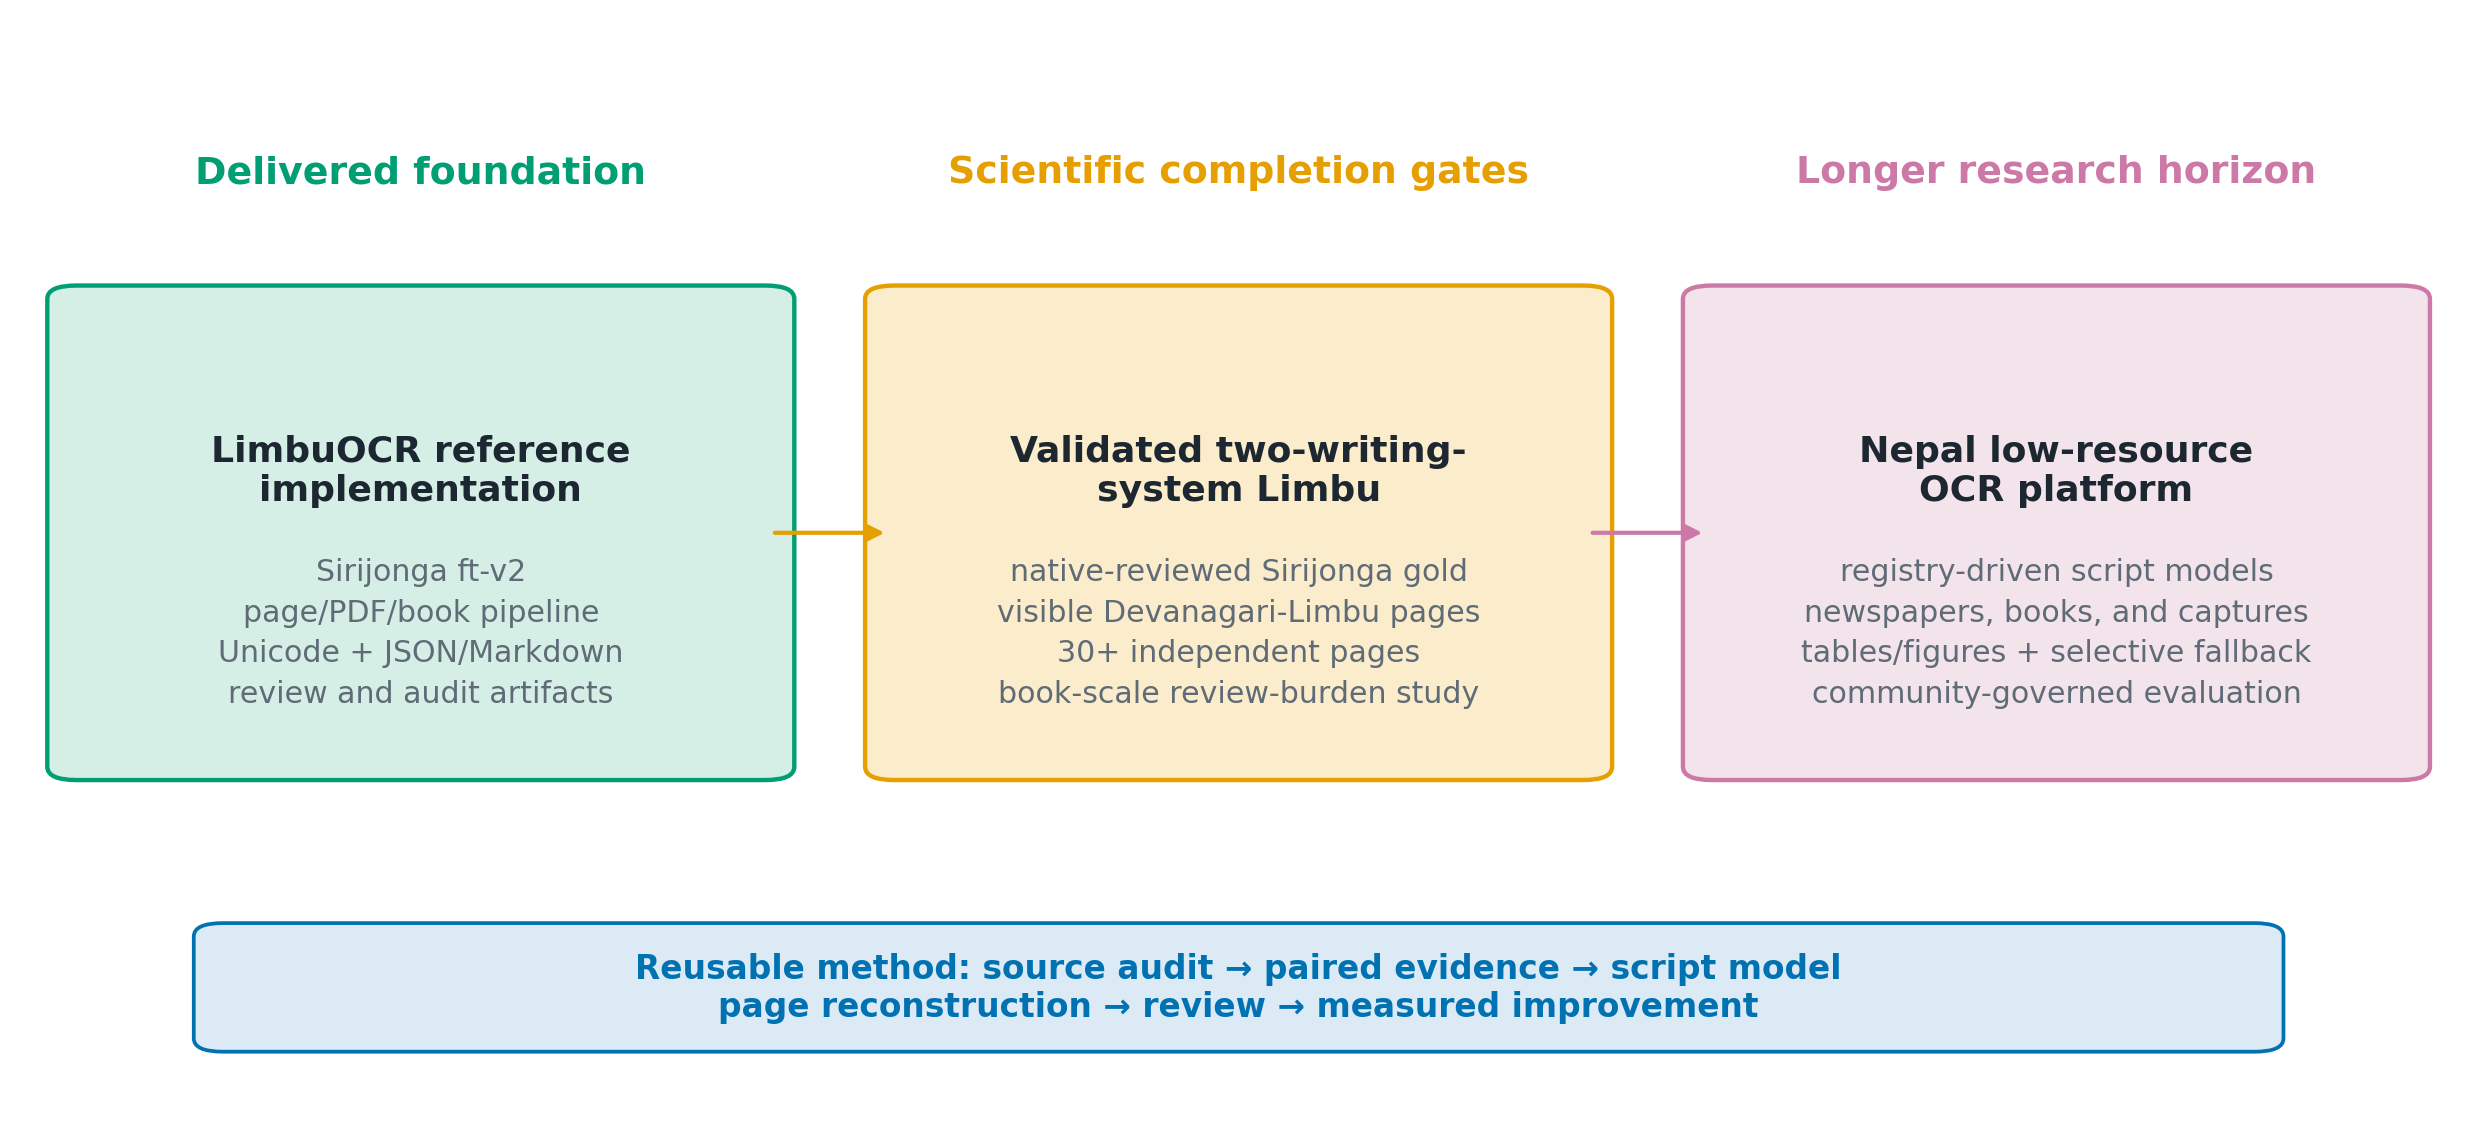
\includegraphics[width=1\linewidth,height=\textheight,keepaspectratio]{figures/research-program.png}
\caption{The research trajectory. LimbuOCR is the delivered reference
implementation; complete two-writing-system Limbu and lower human review
burden are the immediate scientific gates, while transfer to other Nepal
writing systems is a longer horizon rather than a result claimed here.}
\end{figure}

\begin{multicols}{2}

\subsection{2. Limbu OCR as a System
Problem}\label{limbu-ocr-as-a-system-problem}

\subsubsection{2.1 Language, visual script, and output
encoding}\label{language-visual-script-and-output-encoding}

Project sources use both Limbu and Yakthung for the language, and both
Sirijonga and Devanagari for its written form. The Unicode Standard
calls the first of those the Limbu script, records Sirijanga as another
name, and assigns it U+1900--U+194F (Unicode Consortium 2025a). An OCR
record therefore needs at least three separate fields:

\begin{itemize}
\tightlist
\item
  \textbf{language:} the linguistic content is Limbu;
\item
  \textbf{visual writing system:} the page glyphs are Sirijonga or
  Devanagari; and
\item
  \textbf{transcription encoding:} the desired output may reproduce the
  visible script or intentionally transcribe it into another script.
\end{itemize}

For an ordinary OCR benchmark, the reference should use the writing
system visible in the pixels. A Sirijonga page paired with a Devanagari
transcription is a valid cross-script transcription task, but it says
nothing about recognizing Devanagari glyphs. The distinction changes the
dictionary, recognition head, fonts, input profile, and error analysis;
it is not just a naming preference.

Historical PDFs add one more complication. A page may look like
Sirijonga even though its text layer contains Latin or private codes
rendered through an embedded font. A known font map can convert those
codes to Unicode, producing a useful silver label. It does not change
what is on the page: the visible script is still Sirijonga, and the
deployed OCR model still reads pixels.

\subsubsection{2.2 Support maturity}\label{support-maturity}

We use four support levels throughout the paper:

\end{multicols}

\begin{longtable}[]{@{}
  >{\raggedright\arraybackslash}p{(\linewidth - 6\tabcolsep) * \real{0.2500}}
  >{\raggedright\arraybackslash}p{(\linewidth - 6\tabcolsep) * \real{0.2500}}
  >{\raggedright\arraybackslash}p{(\linewidth - 6\tabcolsep) * \real{0.2500}}
  >{\raggedright\arraybackslash}p{(\linewidth - 6\tabcolsep) * \real{0.2500}}@{}}
\toprule\noalign{}
\begin{minipage}[b]{\linewidth}\raggedright
Level
\end{minipage} & \begin{minipage}[b]{\linewidth}\raggedright
Requirement
\end{minipage} & \begin{minipage}[b]{\linewidth}\raggedright
Sirijonga state
\end{minipage} & \begin{minipage}[b]{\linewidth}\raggedright
Visibly Devanagari-written Limbu state
\end{minipage} \\
\midrule\noalign{}
\endhead
\bottomrule\noalign{}
\endlastfoot
Runtime & A model bundle loads and emits text & Present & Present
through generic \texttt{deva-v2} route \\
Operational & Page/book workflow emits structured, reviewable artifacts
& Present & Route is wired into the same workflow \\
Measured & Quality is evaluated on relevant real pixels and references &
Date-disjoint real-print silver diagnostics & Not established on a
verified page set \\
Claim-grade & Frozen, rights-cleared, sufficiently large, human-reviewed
evaluation & Not yet & Not yet \\
\end{longtable}

\begin{multicols}{2}

This vocabulary keeps ``supported'' from doing too much work. Sirijonga
has a measured route; Devanagari has only a working route. Neither has
the human-reviewed, multi-source benchmark needed for a broad accuracy
statement.

\subsubsection{2.3 Design principles}\label{design-principles}

Five choices shape the system.

First, we evaluate the \textbf{page and book} as well as the recognizer.
Cropped-line CER isolates recognition, but a useful system also has to
find, retain, order, and assemble those lines.

Second, the normal route is \textbf{Paddle-first and local-first}: a
compact detector feeds script-specific recognizers. Larger document or
vision-language models may later act as teachers or selective fallbacks.
Their use must be reported so that it does not mask the behavior of the
local engine.

Third, every correction keeps its \textbf{provenance}. Source documents,
rendered and prepared pages, detector boxes, crops, models,
configurations, predictions, and reviewer decisions all retain stable
identities.

Fourth, uncertain output becomes \textbf{visible review work}. Weak
text, empty-looking detections, mixed scripts, and suspicious layout
gaps appear in queues and dashboards. A filter is treated as a
diagnostic until an audit shows that the excluded regions are not text.

Finally, the evaluation is deliberately conservative. We score
machine-converted silver without calling it human ground truth; report
line and page results separately; and make source grouping, leakage
checks, normalization, missing predictions, and reading order part of
the metric definition.

\subsection{3. Related Work}\label{related-work}

\subsubsection{3.1 OCR engines and document
pipelines}\label{ocr-engines-and-document-pipelines}

Tesseract remains a useful example of how segmentation and recognition
meet in a deployable OCR engine (Smith 2007). LimbuOCR instead uses
PaddleOCR as its trainable base. PP-OCR combines lightweight visual
backbones, sequence modeling, and recognition heads intended for
deployment (Li et al. 2022), and PaddleOCR 3.0 extends the surrounding
document-analysis stack (Cui et al. 2025). The recognizer measured here
is the PP-OCRv5 mobile model: a PPLCNetV3 backbone, an SVTR neck, and
CTC/NRTR training heads.

Connectionist Temporal Classification supports sequence recognition
without character-level alignment (Graves et al. 2006), but it does not
solve page layout. Detection, cropping, region selection, and reading
order can spoil assembled text even when pre-cropped lines are
recognized well. We therefore keep line CER, detection F1, matched-line
recognition, and full-page CER separate.

\subsubsection{3.2 Low-resource scripts and synthetic
data}\label{low-resource-scripts-and-synthetic-data}

For a low-resource script, model size is often less limiting than fonts,
standardized text, data rights, training images, and representative
evaluation. Agarwal and Anastasopoulos place these resource gaps at the
center of their survey (Agarwal and Anastasopoulos 2024). Synthetic
rendering can broaden glyph and degradation coverage, while
glyph-centered contrastive learning offers another option when real data
are scarce (Sharma et al. 2024). Neither establishes performance on a
photographed book or an old newspaper.

We use synthesis for coverage and keep the real-page diagnostic
separate. That choice is empirical. In earlier ablations, extra
synthetic and Unicode-coverage rows hurt the frozen real-print score
when the working recognition head was not preserved. Expanding the
dictionary during a warm start resized the output head and failed
outright. The number of rendered lines, by itself, was a poor guide to
model quality.

\subsubsection{3.3 Evaluation, Unicode, and evidence
documentation}\label{evaluation-unicode-and-evidence-documentation}

Unicode normalization and segmentation change what an OCR error count
means. Because Limbu combining signs can split one perceived character
across several codepoints, we report NFC codepoint CER and
extended-grapheme-cluster CER under the Unicode segmentation model
(Unicode Consortium 2025b), plus exact-line accuracy.

Datasets and models are also evidence objects in this project.
Datasheets provide a model for recording collection, composition,
processing, and intended use (Gebru et al. 2021); model cards do the
same for artifact identity, evaluation conditions, limitations, and
deployment (Mitchell et al. 2019). Here those records decide whether a
number can be reproduced, whether pixels can be released, and whether a
later correction still points to its source.

\subsubsection{3.4 Limbu digital heritage and human-in-the-loop
platforms}\label{limbu-digital-heritage-and-human-in-the-loop-platforms}

Research on Yakthung digital heritage places script support inside
community-controlled tools for recording language, stories, and
knowledge (Limbu 2024). Unicode makes Sirijonga text interoperable, but
it does not recognize a page, recover its layout, or help someone
correct the output. Our focused literature search found no peer-reviewed
public Sirijonga page-to-book benchmark with comparable line, page, and
artifact reporting. We accordingly describe ft-v2 as an internal silver
baseline, without a priority or state-of-the-art claim.

Historical-document platforms are the closest systems precedent.
Transkribus joins recognition, transcription, model training, and
archive access in one scholarly workflow (Mühlberger et al. 2019). Work
on postediting likewise argues for transparent suggestions that remain
under human control (Poncelas et al. 2020). LimbuOCR follows that
platform model for printed Limbu, with crop provenance,
two-writing-system evidence, missed-line review, and correction time
treated as explicit research questions.

\subsection{4. The LimbuOCR Platform}\label{the-limbuocr-platform}

LimbuOCR separates model development from book processing. The offline
path turns audited sources and accepted corrections into datasets,
models, and evaluation records. The runtime path turns page pixels into
editable text and review tasks. Human decisions, attached to their
crops, connect the two.

\end{multicols}

\begin{figure}
\centering
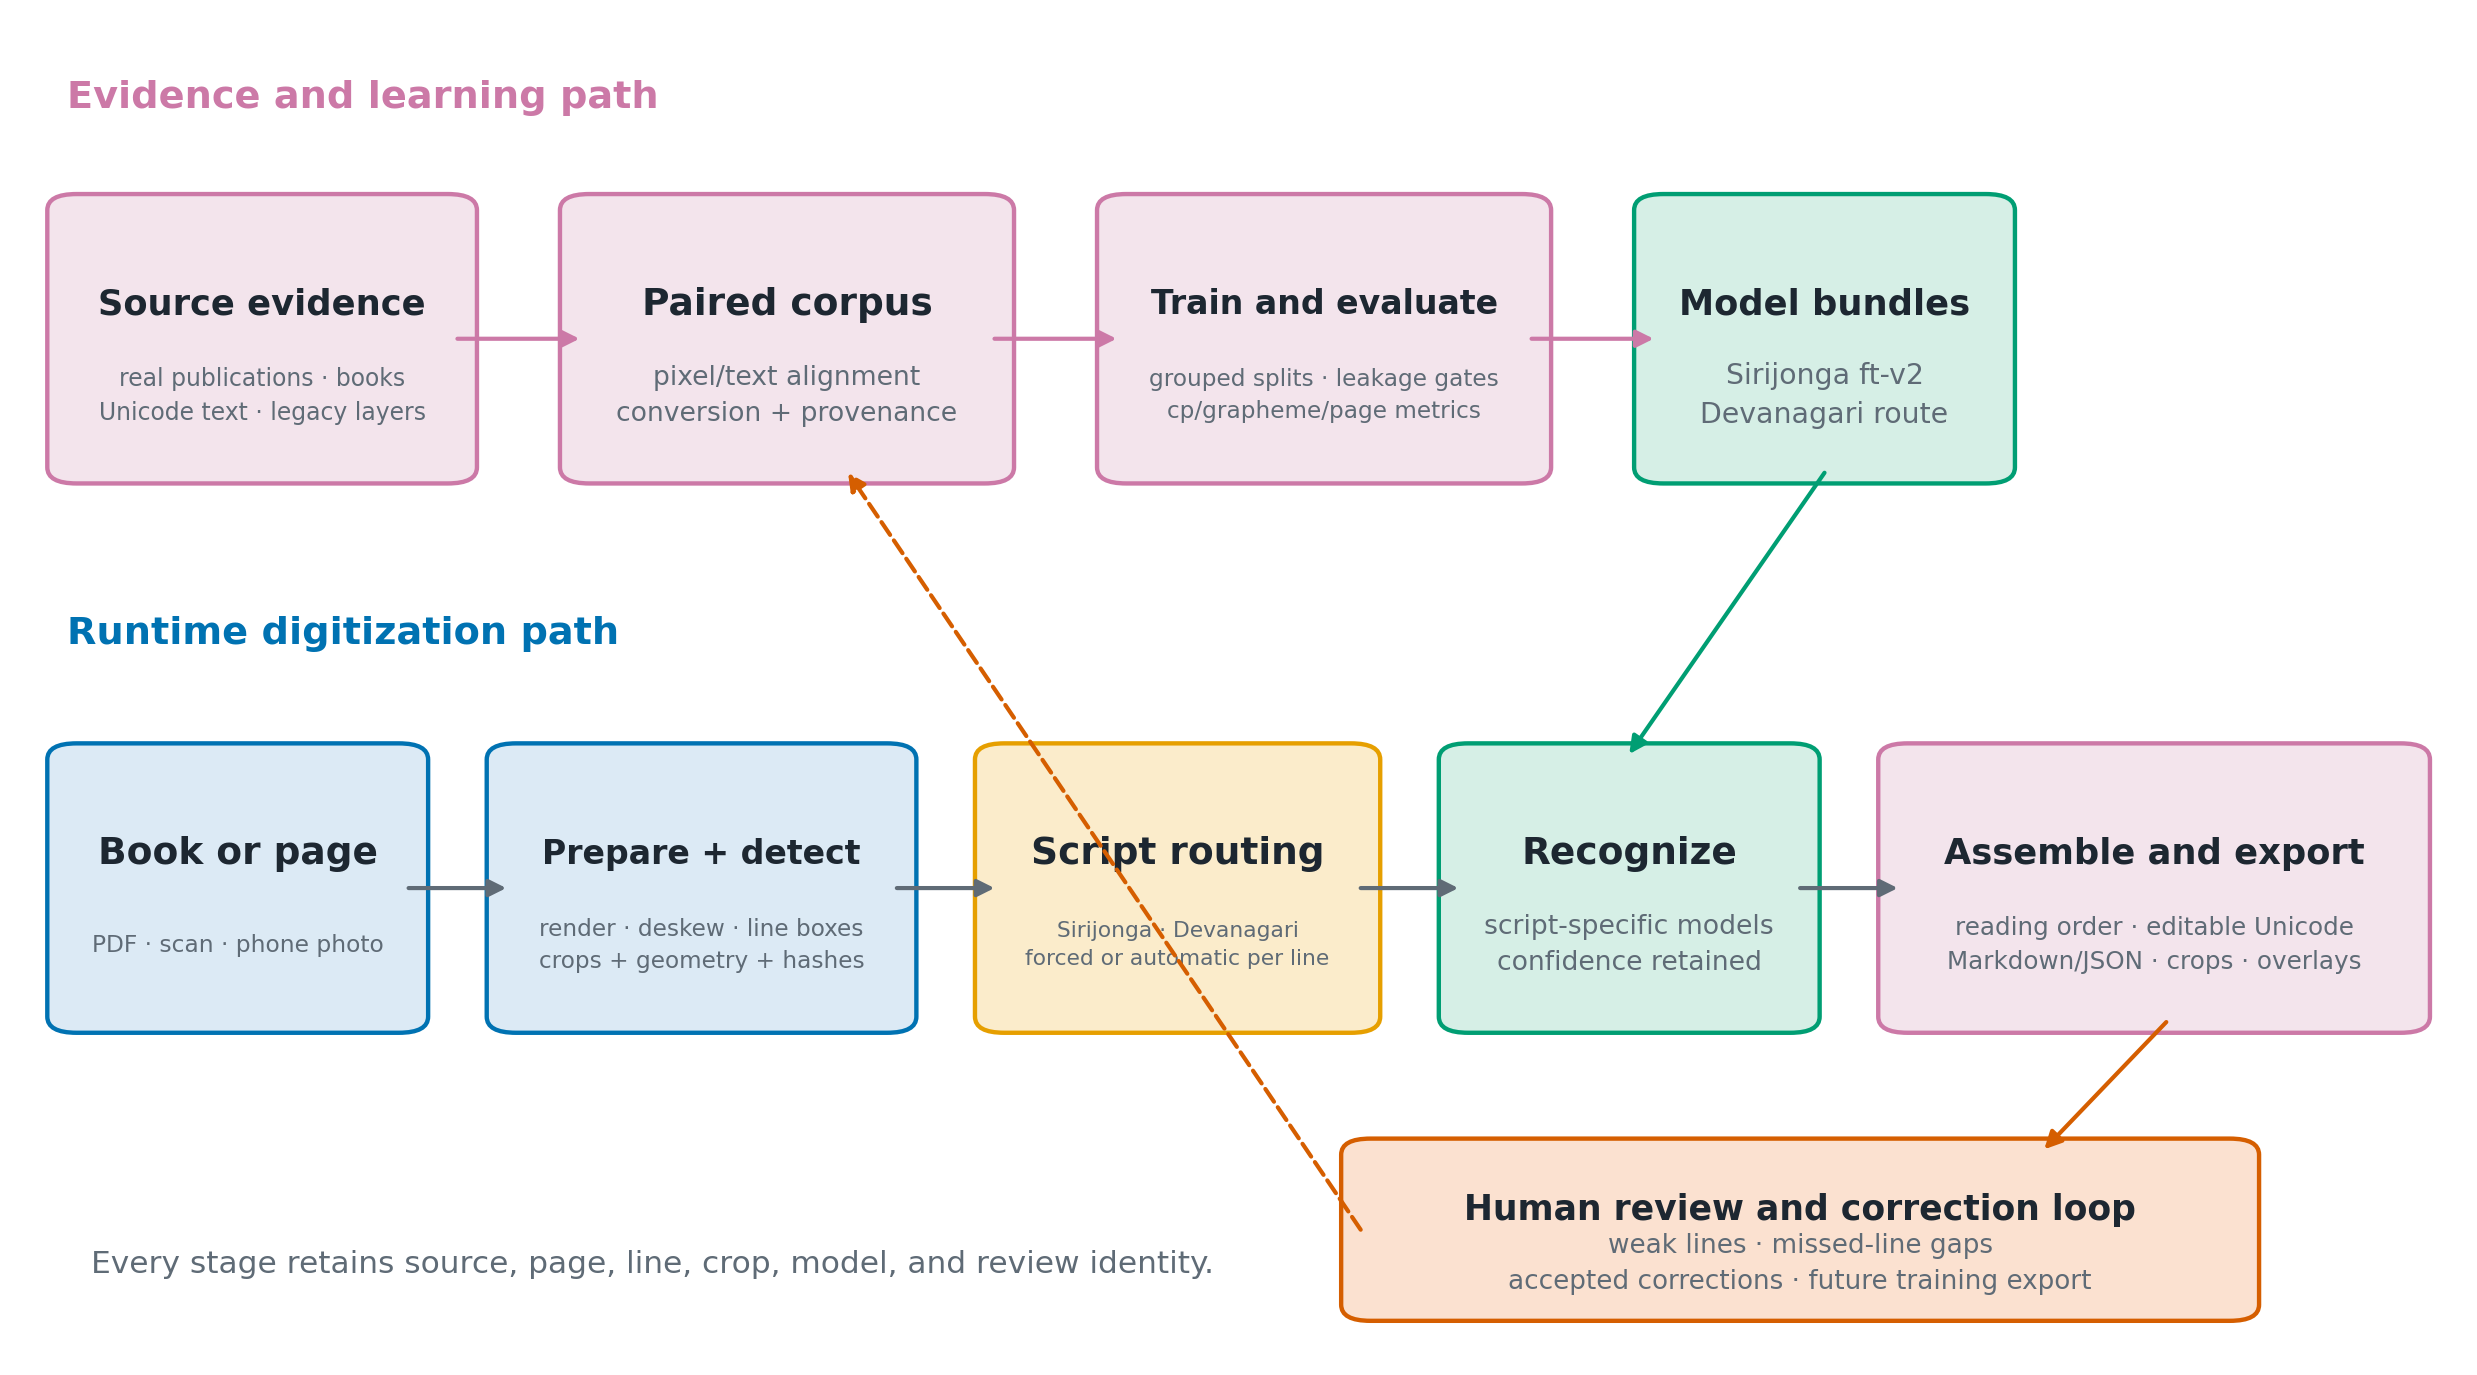
\includegraphics[width=1\linewidth,height=\textheight,keepaspectratio]{figures/system-architecture.png}
\caption{LimbuOCR system architecture. The upper path constructs and
validates evidence and model bundles; the lower path performs
page-to-book OCR. Review decisions remain attached to source crops and
can feed later audited training exports.}
\end{figure}

\begin{multicols}{2}

\subsubsection{4.1 Intake and capture
preparation}\label{intake-and-capture-preparation}

The runtime accepts a line crop, a full page, an ordered image set, or a
PDF. PDF pages are rendered at a recorded resolution. For photographs,
the broader repository workflow can rotate, deskew, crop, and correct
perspective while retaining hashes of the raw and prepared images. It
also flags duplicates, non-target pages, low-information captures, and
likely recaptures.

Video stays outside the OCR boundary until a stable page frame has been
chosen. This lets us inspect capture quality before blaming the
recognizer for errors introduced during frame selection.

\subsubsection{4.2 Text-line detection and crop
identity}\label{text-line-detection-and-crop-identity}

The compact application uses PaddleOCR to detect text on a full page.
Each polygon becomes a crop with page-relative geometry and the
prototype's seed OCR score; the selected recognizer adds its own
confidence later. A morphology- based line detector is available for
rescue cases and controlled comparisons. A YOLO detector is retained
only as a diagnostic probe.

The crop is the smallest reviewable evidence unit. Its record links the
source page, prepared page, detector box, image, recognizer output, and
final book line. A missed line, extra region, or wrong character can
therefore be traced to the stage that produced it.

\subsubsection{4.3 Script-aware
recognition}\label{script-aware-recognition}

Recognition may be fixed to Sirijonga or Devanagari, or chosen
automatically for each crop. The local application bundles:

\begin{itemize}
\tightlist
\item
  \texttt{limbu-sirijonga-ft-v2}, the measured Sirijonga recognizer
  described in this paper; and
\item
  \texttt{deva-v2}, a generic Devanagari recognizer that supplies the
  runtime route but is not a Limbu-specific Devanagari accuracy result.
\end{itemize}

Automatic mode compares script evidence in the candidate readings.
Routing is separate from the model bundles, so a later Limbu-specific
Devanagari model can replace the generic recognizer without changes to
page intake or export.

\subsubsection{4.4 Reading order and book
assembly}\label{reading-order-and-book-assembly}

Detection produces regions, not a readable document. LimbuOCR can
assemble them by row or by column; the six-column newspaper test uses
deterministic column-major order. The selected rule is saved with both
output and score. As Section 8 shows, page edit distance is
uninterpretable when reference and hypothesis use different
linearizations.

For a page sequence, the system writes page and book text without losing
page breaks. The compact application packages \texttt{book.txt},
\texttt{book.json}, annotated pages, and line crops in one archive. The
repository workflow adds Markdown projections, page manifests,
layout-gap records, and document JSON accepted by the scorer.

\subsubsection{4.5 Review, correction, and the learning
loop}\label{review-correction-and-the-learning-loop}

A confidence number is not, by itself, a review workflow. LimbuOCR
places weak lines in page order and shows each prediction beside its
crop, confidence, and page context. Low-confidence text, empty
detections, likely page furniture, mixed scripts, and vertical gaps that
may contain missed lines receive separate queue entries.

Corrections fail closed: the tooling checks source and crop identities
before accepting an edit, records changed rows, and regenerates the
book. A training export includes only non-empty text that a reviewer
explicitly accepted. Machine context and automatic prefill remain
suggestions. Mechanical smoke tests cover this chain, but fluent
reviewers have not completed the large Limbu packets. The software is
present; evidence about review quality and effort is not.

\subsubsection{4.6 Reusability beyond one
script}\label{reusability-beyond-one-script}

Capture preparation, detection, crop identity, assembly, export, and
review do not depend much on the language. Script ranges, dictionaries,
model bundles, and converters do. A shared Unicode-block table
identifies scripts, while a configuration-driven runner resolves each
language's detector, recognizers, converters, and writing-system
profiles from a 50-language pipeline registry. Given a PDF or ordered
image directory, it writes structured page records, book text and
Markdown, a review queue, and a hash-bearing run summary.

Registration does not grant permission to run. Every recognizer is
marked \texttt{champion}, \texttt{diagnostic-only}, \texttt{blocked}, or
\texttt{failed-fit}, and an execution allowlist decides which statuses
may enter the production path. A withdrawn or legally blocked model
stays visible for audit but will not execute there. Section 10 gives the
evidence behind these statuses. At this stage the reusable software is
implemented; quality transfer is measured only for the diagnostic
reported in that section.

\subsection{5. Building Real-Print Sirijonga
Evidence}\label{building-real-print-sirijonga-evidence}

\subsubsection{5.1 Authoritative source
pairing}\label{authoritative-source-pairing}

The real-print material comes from Limbu pages in the \emph{Naya Nepal}
supplement of Gorkhapatra epaper PDFs. A publication landing page tells
us which language and date to look for; it supplies no training text.
Both sides of every pair come from the full PDF. We render the page
image and extract the text layer from that same page.

That same-page rule prevents a subtle mismatch: a news-card thumbnail
may not contain the article text displayed beside it on the website.
Each retained row therefore records the PDF and its hash, page number,
rendered page, line geometry, raw codes, converted text, and crop. We
manually checked the test page dated 2082-08-12; it is a six-column
Sirijonga newspaper page, and the source-verification report records its
rendered-image SHA-256. We do not reproduce publisher pixels because the
current owner determination covers derived counts and metrics, while
redistribution still awaits a formal license statement.

\subsubsection{5.2 Legacy-font recovery as a data
method}\label{legacy-font-recovery-as-a-data-method}

The pages display Sirijonga through Namdhinggo-family fonts, but their
text layers are not Unicode Limbu. During extraction we group PDF spans
into lines and convert the stored codes with \texttt{Limbu.map}. The
Unicode label and its image crop consequently trace back to one PDF
layout object.

The pairing scales, but it is not gold ground truth. Font maps can be
wrong; PDF spans may arrive out of order, split, or disappear; and our
own grouping and normalization can introduce errors. Every row is
therefore marked \texttt{pdf\_text\_layer\_silver} and excluded from
claim-grade evidence. The text layer is used to build and evaluate data,
never as runtime input to the recognizer.

\subsubsection{5.3 Grouped splitting and leakage
control}\label{grouped-splitting-and-leakage-control}

The rebuilt collection contains 4,872 non-empty line pairs from 16
publication dates. We keep every line from a date in the same split.
After sorting the dates, indices congruent to 2 modulo 5 go to test,
indices congruent to 0 go to development, and the rest go to training.
The test dates are 2082-03-24, 2082-08-12, and 2082-12-25.

We then remove normalized labels that repeat across split boundaries.
The 38 excluded rows leave 4,834 lines: 2,711 for training from nine
dates, 1,221 for development from four dates, and 902 for testing from
three dates. Date grouping stops same-edition leakage, while label
filtering catches exact boilerplate repeated on different dates.
Near-duplicate phrases and shared page templates may remain.

\end{multicols}

\begin{figure}
\centering
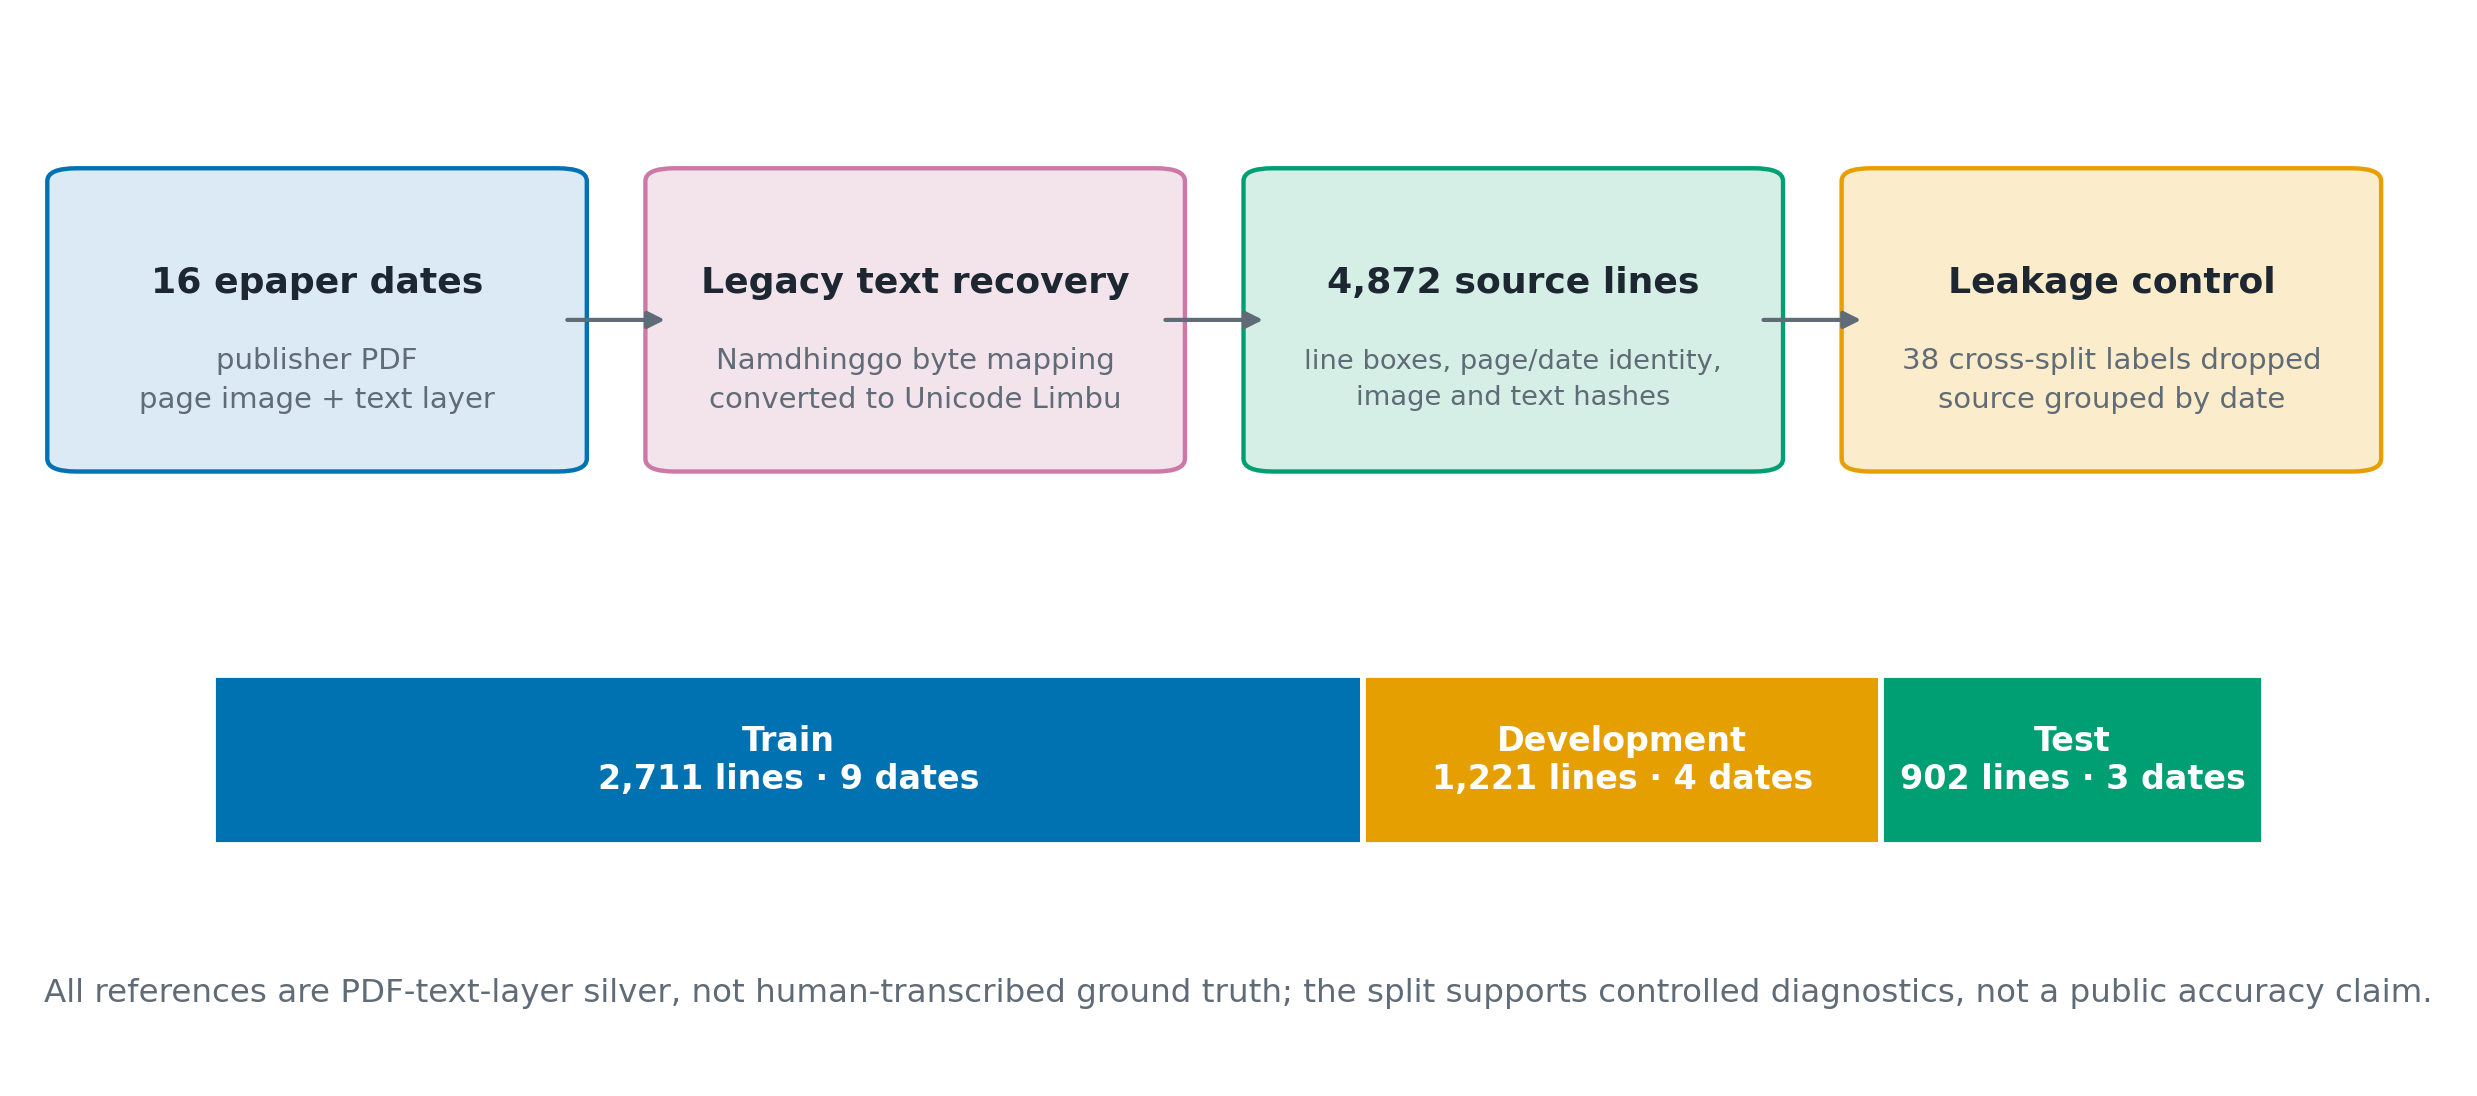
\includegraphics[width=1\linewidth,height=\textheight,keepaspectratio]{figures/limbu-source-evidence.png}
\caption{Construction of the real-print Sirijonga evidence. The figure
is generated from the pack summary and contains no publisher pixels.
Same-PDF pairing and date grouping make the diagnostic reproducible; the
references remain machine-converted silver.}
\end{figure}

\begin{multicols}{2}

\subsubsection{5.4 Training mixture}\label{training-mixture}

The ft-v2 training bundle has 46,753 training rows and 1,221 development
rows. Training combines 25,065 synthetic examples with eight passes over
the 2,711 real-print lines. Another 3,090 referenced synthetic images
were lost in a storage failure; we excluded them instead of recreating
different bytes under the old names. Replay changes optimization weight,
not sample independence: the real portion still contains only 2,711
distinct lines.

The training bundle, YAML, log, selected checkpoint, inference export,
predictions, and scores all survive. Training used an NVIDIA L4 for 40
epochs (about 8.5 GPU-hours), with epoch 39 selected on the development
set. Building this paper checks those artifacts but does not rerun
training.

\subsection{6. Model and Evaluation
Method}\label{model-and-evaluation-method}

\subsubsection{6.1 Sirijonga recognizer}\label{sirijonga-recognizer}

We initialize the recognizer from PaddleOCR's pretrained PP-OCRv5 mobile
checkpoint. Its PPLCNetV3 backbone runs at scale 0.95, followed by an
SVTR neck and CTC/NRTR heads. Inputs are 48 by 320 pixels and may
contain at most 128 characters. We train for 40 epochs with Adam, a
cosine schedule from \(10^{-4}\), one warm-up epoch, and batches of 64.
The output dictionary remains the working
\texttt{limbu-sirijonga-v2.txt} from the previous system.

Our comparator is the preceding real-heavy Sirijonga export. We run both
models through one local CPU inference and scoring path on the same 902
images and references. ft-v2 never sees its test dates during training
or selection. The older model may have seen some of them, because its
training history cannot be isolated to the same standard. This is an
engineering before/after comparison, not a controlled leaderboard
between two equally separated training regimes.

\subsubsection{6.2 Line metrics}\label{line-metrics}

We normalize strings to NFC and preserve whitespace. For reference \(r\)
and prediction \(p\), CER is their Levenshtein distance divided by the
length of \(r\). Codepoint and extended-grapheme CER are micro-averaged:
edits and reference lengths are summed before division, so longer lines
carry proportionally more weight. Exact-line accuracy counts normalized
predictions that match the entire reference.

Each view catches something different. Codepoint CER exposes encoding
edits; grapheme CER groups perceived characters; and exact-line accuracy
fails on a single punctuation, spacing, or combining-sign difference.

\subsubsection{6.3 Non-oracle page
evaluation}\label{non-oracle-page-evaluation}

A page run starts with the complete rendered image. The detector
proposes line regions, the recognizer reads each crop, configured
low-value outputs are filtered, and the remaining boxes are ordered by
column. The one-to-one matcher pairs a prediction with a reference at
bounding-box intersection-over-union of at least 0.5.

We report:

\begin{itemize}
\tightlist
\item
  detection precision, recall, and F1 from reference, predicted, and
  matched line counts;
\item
  codepoint and grapheme CER over the fully assembled page text;
\item
  CER and exact accuracy over geometrically matched lines; and
\item
  missed and unmatched line counts.
\end{itemize}

The 16-page regression set catches deployment regressions, but 13 of its
dates also occur in ft-v2 training or development. For a cleaner check,
we rescore the already exported documents for the three line-test dates.
Those pages contain 907 reference lines and are date-disjoint from model
selection. They are still only three pages from one publisher, with
references derived by the same silver process as the line test.

\subsubsection{6.4 Evidence status}\label{evidence-status}

We do not present these page results as accuracy claims, for four
reasons: no human review, only three independent pages rather than the
project's minimum of 30, no permission to redistribute the pixels, and
no complete multi-domain leakage and source-independence audit. We
report them as diagnostics because they are reproducible and show where
the system is failing; they do not support a broad accuracy claim.

\subsection{7. Results}\label{results}

\subsubsection{7.1 Date-disjoint line
recognition}\label{date-disjoint-line-recognition}

\end{multicols}

\begin{longtable}[]{@{}
  >{\raggedright\arraybackslash}p{(\linewidth - 8\tabcolsep) * \real{0.1579}}
  >{\raggedleft\arraybackslash}p{(\linewidth - 8\tabcolsep) * \real{0.2105}}
  >{\raggedleft\arraybackslash}p{(\linewidth - 8\tabcolsep) * \real{0.2105}}
  >{\raggedleft\arraybackslash}p{(\linewidth - 8\tabcolsep) * \real{0.2105}}
  >{\raggedleft\arraybackslash}p{(\linewidth - 8\tabcolsep) * \real{0.2105}}@{}}
\toprule\noalign{}
\begin{minipage}[b]{\linewidth}\raggedright
Recognizer
\end{minipage} & \begin{minipage}[b]{\linewidth}\raggedleft
Lines
\end{minipage} & \begin{minipage}[b]{\linewidth}\raggedleft
Codepoint CER
\end{minipage} & \begin{minipage}[b]{\linewidth}\raggedleft
Grapheme CER
\end{minipage} & \begin{minipage}[b]{\linewidth}\raggedleft
Exact-line accuracy
\end{minipage} \\
\midrule\noalign{}
\endhead
\bottomrule\noalign{}
\endlastfoot
Previous real-heavy export & 902 & 1.379\% & 2.840\% & 63.75\% \\
ft-v2 & 902 & \textbf{0.474\%} & \textbf{0.979\%} & \textbf{85.92\%} \\
\end{longtable}

\begin{multicols}{2}

The 902 test lines contain 34,814 codepoints and 16,760 grapheme
clusters. Against the previous export, ft-v2 cuts codepoint CER by
65.625\% and grapheme CER by 65.55\%; exact-line accuracy gains 22.17
percentage points. This measures agreement with the same-PDF silver
layer, not with a fluent transcription.

\end{multicols}

\begin{figure}
\centering
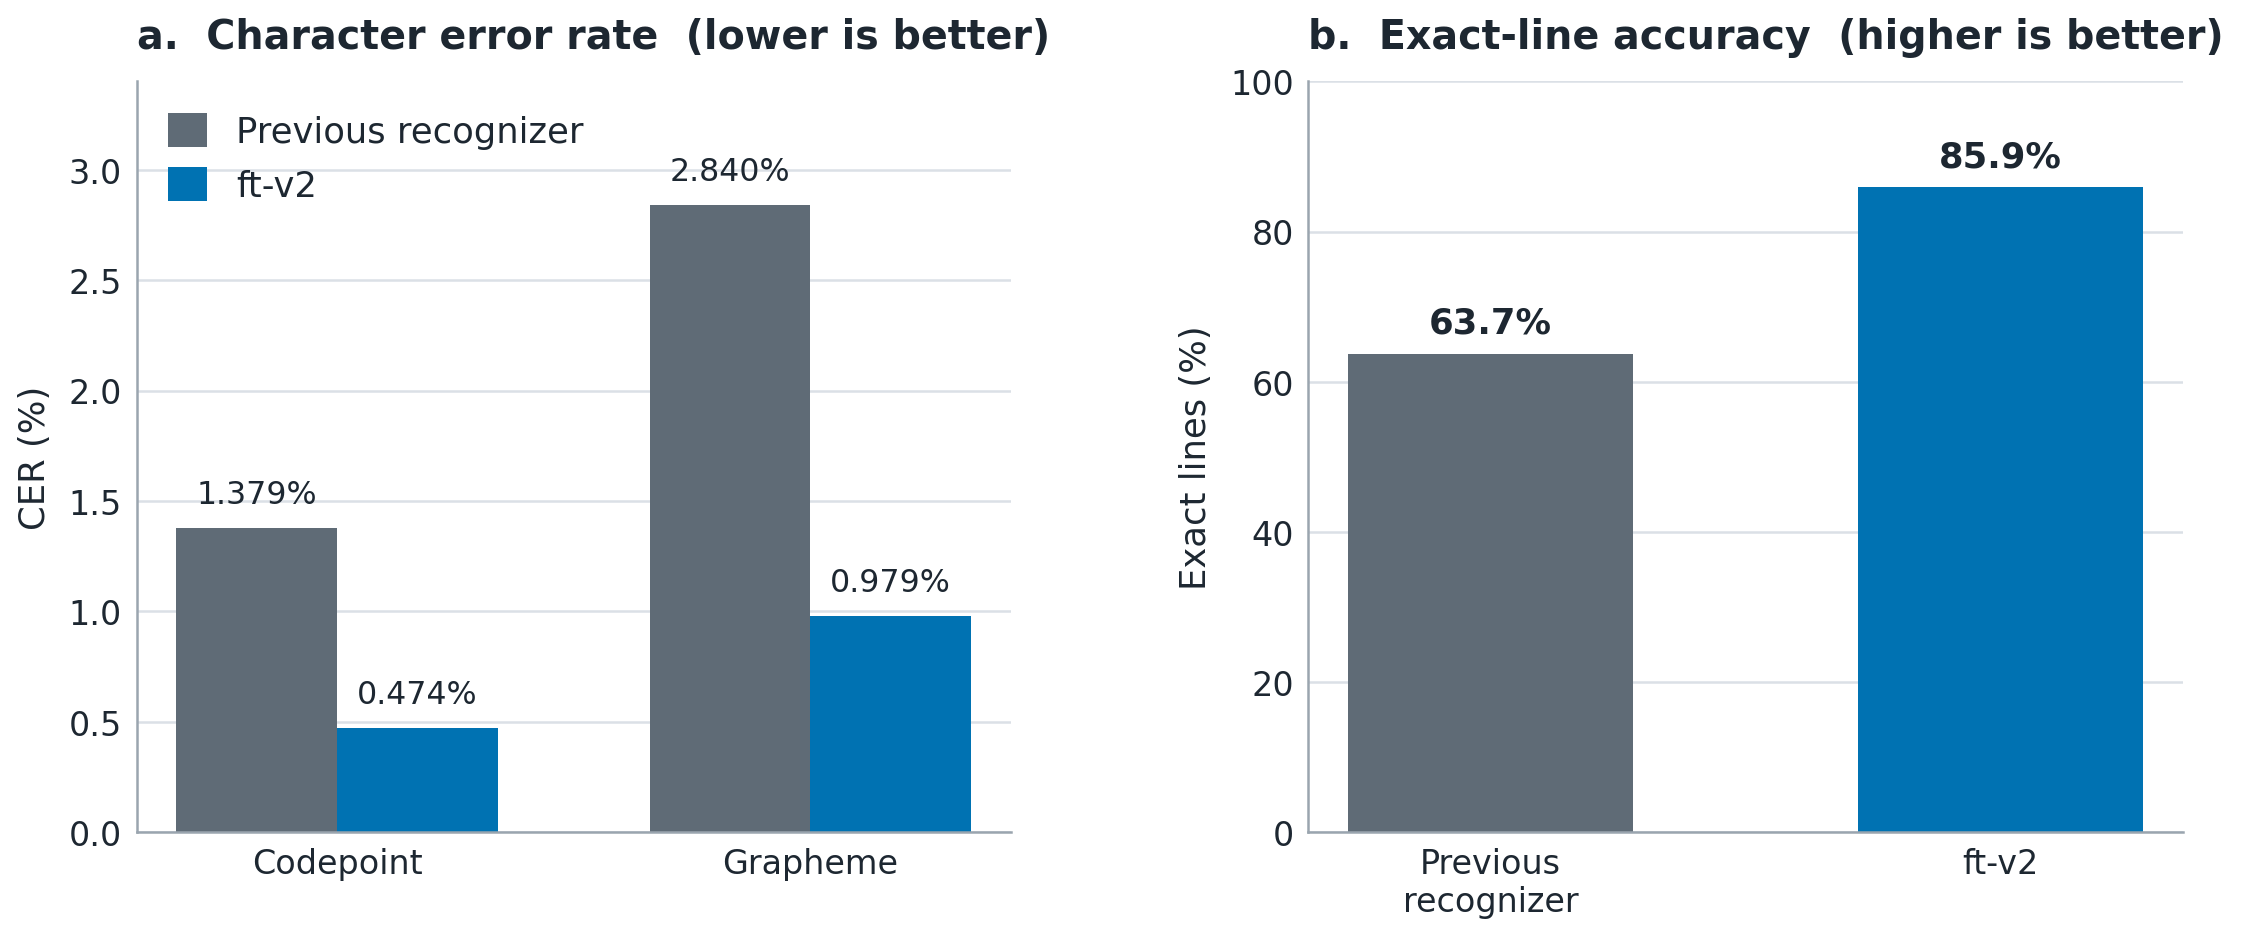
\includegraphics[width=0.98\linewidth,height=\textheight,keepaspectratio]{figures/limbu-recognizer-results.png}
\caption{Sirijonga recognition on the same date-separated silver test
(902 lines, 34,814 codepoints, 16,760 grapheme clusters). Error and
exact-line accuracy are shown separately because their preferred
directions differ; the references remain machine-converted silver.}
\end{figure}

\begin{multicols}{2}

For RQ1, the result shows that same-source pairing can yield a useful
internal baseline when transcription is scarce. Date grouping, real-line
replay, and a fixed dictionary outperform the preceding deployment on
this print register. Only native review can tell us how much of the
residual error---and how much of the apparent agreement---belongs to the
silver labels.

\subsubsection{7.2 Non-oracle pages on the held-out
dates}\label{non-oracle-pages-on-the-held-out-dates}

\end{multicols}

\begin{longtable}[]{@{}
  >{\raggedright\arraybackslash}p{(\linewidth - 14\tabcolsep) * \real{0.0968}}
  >{\raggedleft\arraybackslash}p{(\linewidth - 14\tabcolsep) * \real{0.1290}}
  >{\raggedleft\arraybackslash}p{(\linewidth - 14\tabcolsep) * \real{0.1290}}
  >{\raggedleft\arraybackslash}p{(\linewidth - 14\tabcolsep) * \real{0.1290}}
  >{\raggedleft\arraybackslash}p{(\linewidth - 14\tabcolsep) * \real{0.1290}}
  >{\raggedleft\arraybackslash}p{(\linewidth - 14\tabcolsep) * \real{0.1290}}
  >{\raggedleft\arraybackslash}p{(\linewidth - 14\tabcolsep) * \real{0.1290}}
  >{\raggedleft\arraybackslash}p{(\linewidth - 14\tabcolsep) * \real{0.1290}}@{}}
\toprule\noalign{}
\begin{minipage}[b]{\linewidth}\raggedright
System
\end{minipage} & \begin{minipage}[b]{\linewidth}\raggedleft
Pages
\end{minipage} & \begin{minipage}[b]{\linewidth}\raggedleft
Ref./pred./matched lines
\end{minipage} & \begin{minipage}[b]{\linewidth}\raggedleft
Detection F1
\end{minipage} & \begin{minipage}[b]{\linewidth}\raggedleft
Page cp CER
\end{minipage} & \begin{minipage}[b]{\linewidth}\raggedleft
Page grapheme CER
\end{minipage} & \begin{minipage}[b]{\linewidth}\raggedleft
Matched cp CER
\end{minipage} & \begin{minipage}[b]{\linewidth}\raggedleft
Exact matched lines
\end{minipage} \\
\midrule\noalign{}
\endhead
\bottomrule\noalign{}
\endlastfoot
Previous recognizer & 3 & 907 / 903 / 877 & 96.91\% & 3.957\% & 6.280\%
& 2.569\% & 45.95\% \\
ft-v2 & 3 & 907 / 904 / 877 & 96.85\% & \textbf{2.575\%} &
\textbf{3.361\%} & \textbf{1.012\%} & \textbf{76.17\%} \\
\end{longtable}

\begin{multicols}{2}

The detector is fixed; its small F1 change comes from downstream
filtering. Most of the improvement is in recognition. ft-v2 reduces
assembled-page codepoint error by 34.94\% and grapheme error by 46.49\%
relative to the previous model. Exact accuracy on 877 matched lines
rises by 30.22 percentage points. The run still misses 30 reference
lines and leaves 27 predictions unmatched, so these numbers include more
than oracle-crop recognition.

\end{multicols}

\begin{figure}
\centering
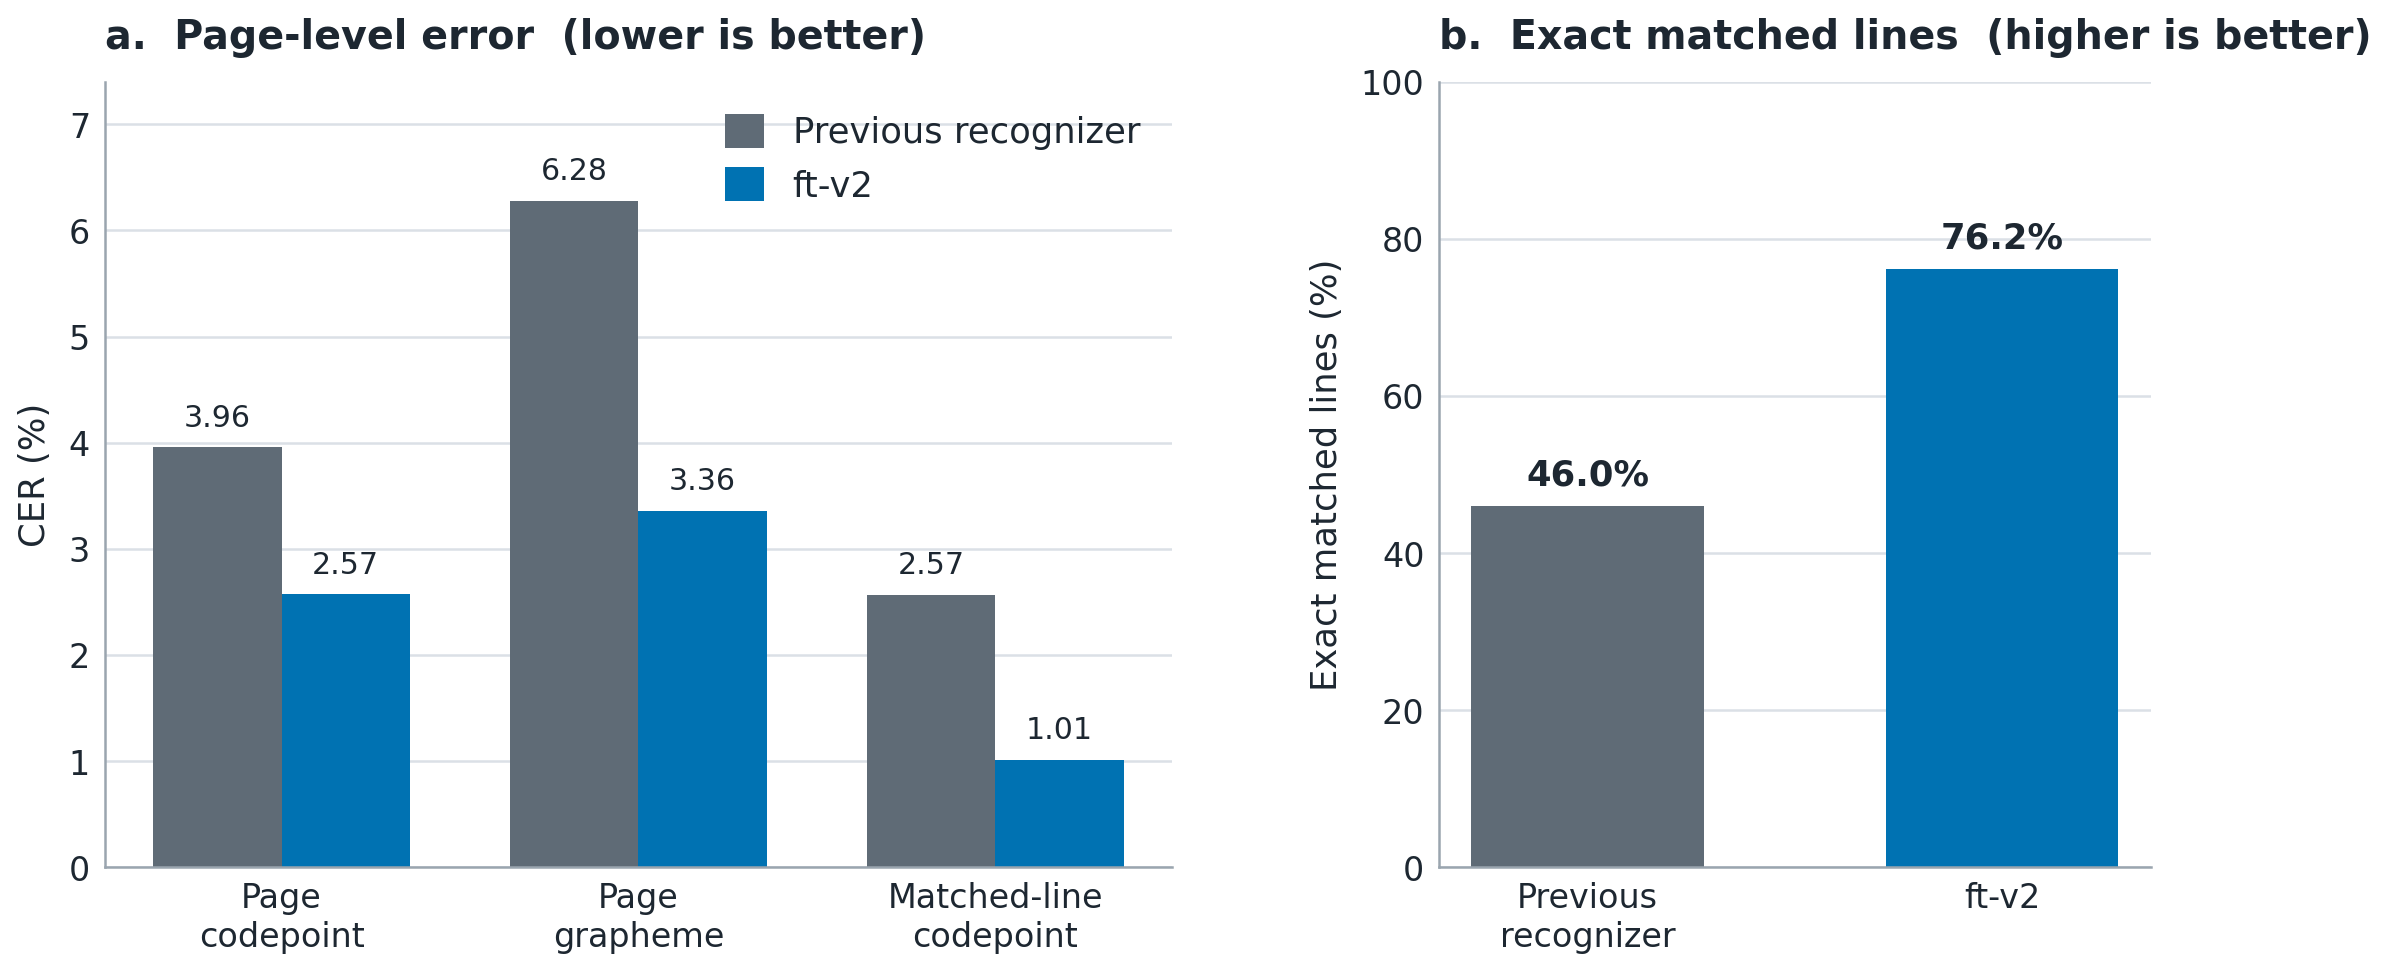
\includegraphics[width=0.98\linewidth,height=\textheight,keepaspectratio]{figures/limbu-page-results.png}
\caption{Non-oracle page results on the three dates reserved by the
recognizer split (3 pages, 907 reference lines, detector F1 96.85\%).
All three error measures share one CER axis; panel b reports exact
matched-line accuracy. The metric contains detection, recognition, and
assembly effects; the references remain silver.}
\end{figure}

\begin{multicols}{2}

\subsubsection{7.3 Sixteen-page regression
check}\label{sixteen-page-regression-check}

\end{multicols}

\begin{longtable}[]{@{}
  >{\raggedright\arraybackslash}p{(\linewidth - 12\tabcolsep) * \real{0.1111}}
  >{\raggedleft\arraybackslash}p{(\linewidth - 12\tabcolsep) * \real{0.1481}}
  >{\raggedleft\arraybackslash}p{(\linewidth - 12\tabcolsep) * \real{0.1481}}
  >{\raggedleft\arraybackslash}p{(\linewidth - 12\tabcolsep) * \real{0.1481}}
  >{\raggedleft\arraybackslash}p{(\linewidth - 12\tabcolsep) * \real{0.1481}}
  >{\raggedleft\arraybackslash}p{(\linewidth - 12\tabcolsep) * \real{0.1481}}
  >{\raggedleft\arraybackslash}p{(\linewidth - 12\tabcolsep) * \real{0.1481}}@{}}
\toprule\noalign{}
\begin{minipage}[b]{\linewidth}\raggedright
System
\end{minipage} & \begin{minipage}[b]{\linewidth}\raggedleft
Pages
\end{minipage} & \begin{minipage}[b]{\linewidth}\raggedleft
Page cp CER
\end{minipage} & \begin{minipage}[b]{\linewidth}\raggedleft
Page grapheme CER
\end{minipage} & \begin{minipage}[b]{\linewidth}\raggedleft
Detection F1
\end{minipage} & \begin{minipage}[b]{\linewidth}\raggedleft
Matched cp CER
\end{minipage} & \begin{minipage}[b]{\linewidth}\raggedleft
Exact matched lines
\end{minipage} \\
\midrule\noalign{}
\endhead
\bottomrule\noalign{}
\endlastfoot
Previous recognizer, shared column-major & 16 & 4.329\% & 6.714\% &
96.57\% & 2.657\% & 43.40\% \\
ft-v2, shared column-major & 16 & \textbf{2.722\%} & \textbf{3.468\%} &
96.50\% & \textbf{0.898\%} & \textbf{79.27\%} \\
\end{longtable}

\begin{multicols}{2}

Across all 16 regression pages, replacing the recognizer helps while
detection and assembly stay fixed. Most page dates also occur in
training or development, so this table is an acceptance check for the
bundled model. It is not an estimate of performance on an unseen book.

\subsection{8. Lessons from the
Experiments}\label{lessons-from-the-experiments}

\subsubsection{8.1 Real-domain weighting matters more than
indiscriminate
synthesis}\label{real-domain-weighting-matters-more-than-indiscriminate-synthesis}

Synthetic data supplied script and glyph coverage, but adding more of it
did not consistently improve real-print OCR. One targeted
synthetic/Unicode expansion made the frozen real-print score worse.
During another warm start, expanding the dictionary replaced part of the
recognition head instead of simply extending it. ft-v2 worked after we
kept the output space fixed and gave the aligned real-print lines much
more replay weight.

Future runs should use synthetic rendering as controlled coverage,
compare it against a fixed real-domain test, and rebuild the head
deliberately whenever the character set changes.

\subsubsection{8.2 Page CER is defined by its serialization
contract}\label{page-cer-is-defined-by-its-serialization-contract}

Full-page CER compares two long strings, so it measures sequence as much
as text. That makes the serialization rule part of the metric
definition. On the 16-page set, the same recognizer output can score
41.34\% codepoint CER when reference and prediction are linearized under
different rules, alongside 4,895 reference lines, 4,839 predictions,
4,700 geometric matches, 96.57\% detection F1, and only 2.66\% CER on
matched lines.

Applying one explicit column-major linearization to both sides resolves
the contradiction: codepoint CER becomes 4.329\% and grapheme CER
6.714\% over the identical 4,839 predictions and 4,700 matched lines,
with no model retrained and no recognized text altered.

\end{multicols}

\begin{figure}
\centering
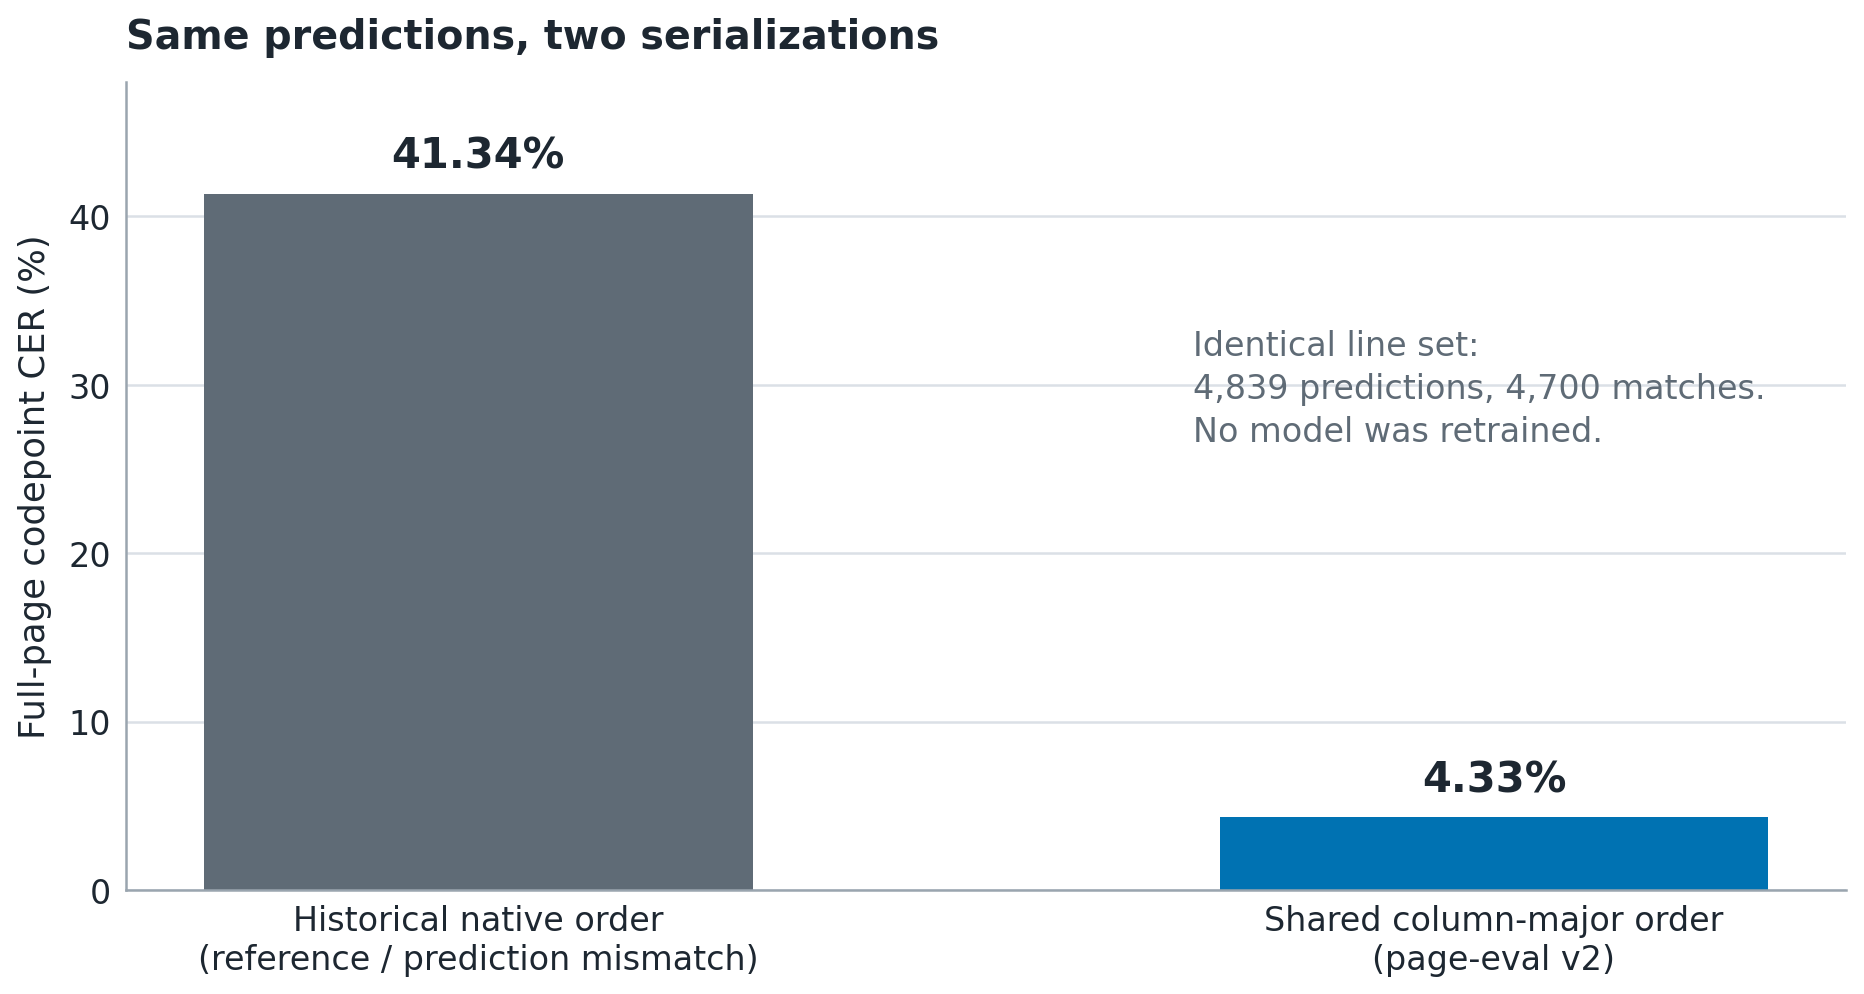
\includegraphics[width=0.82\linewidth,height=\textheight,keepaspectratio]{figures/limbu-linearization-diagnostic.png}
\caption{The same earlier predictions scored under inconsistent
historical serialization and one shared column-major serialization
(identical 4,839 predictions and 4,700 matches; no model retrained).
This is a metric-definition correction, not a model improvement, and v1-
and v2-scale page CER must not be compared directly.}
\end{figure}

\begin{multicols}{2}

Page CER measures sequence as well as text. On a six-column page, a
small vertical offset can cause a global y-sort to weave two columns
together. Edit distance then counts moved blocks as character errors.
For this evaluation, RQ2 has a clear answer: the catastrophic-looking
result came mainly from an inconsistent sequence definition. Once fixed,
the remaining error belongs to recognition, missing and extra lines,
crop quality, and layout rules beyond this newspaper template.

We now record the linearization with every page score and expose
detection, matched-line recognition, and assembled text separately. The
41.34\% and 4.329\% figures describe two evaluations of the same
predictions, not two OCR systems.

\subsubsection{8.3 A target string does not identify the visual writing
system}\label{a-target-string-does-not-identify-the-visual-writing-system}

An early curriculum pack shows why target text alone cannot establish
the page script. We had called the pack Devanagari-written Limbu because
its JSON references contain Devanagari Unicode. On reinspection, the PDF
pixels show Sirijonga/Yakthung glyphs. The fonts include
\texttt{YakthungBold} and \texttt{NamdhinggoSILL}, while raw extraction
yields ASCII-like legacy codes rather than the Devanagari reference.

On the inspected mathematics page, the 14-line reference has 408
Devanagari- block codepoints and no Limbu-block codepoints. The page
itself looks like Sirijonga. The actual task is:

\[\text{Sirijonga-looking pixels} \rightarrow \text{Devanagari transcription}\]

It is not:

\[\text{Devanagari-looking pixels} \rightarrow \text{Devanagari OCR}.\]

A surviving 31-crop diagnostic is evidence about cross-script
transcription, not Devanagari OCR. Its raw scoring bundle was also lost,
which gives us a second reason to omit it from the verified tables.

The audit provides the operational answer to RQ3: future manifests store
\texttt{language}, \texttt{visual\_script}, \texttt{source\_encoding},
and \texttt{transcription\_encoding} as separate fields, and support
maturity remains explicit. We now call \texttt{deva-v2} a generic
runtime route. A Limbu-specific Devanagari result will require visibly
Devanagari pixels containing Limbu, with references checked against
those pixels.

\subsubsection{8.4 Review burden is the next system
metric}\label{review-burden-is-the-next-system-metric}

None of the recognition scores tells us how long a book takes to
correct. Low average CER can coexist with missing headings, confidently
wrong lines, or an interface that makes the editor search the source
page for every error. A higher raw CER may be tolerable when uncertain
regions arrive with reliable crops and reading context.

The RQ4 study should measure lines routed to review, missing and extra
lines, correction time per page and per thousand characters, accuracy
after a bounded review, and the share of a book that needs
resegmentation or recapture. Those measures, rather than CER alone, will
decide whether the system is useful in production.

\subsection{9. What Is Implemented}\label{what-is-implemented}

The repository contains both a compact Limbu OCR application and the
larger workflow used for these experiments. Its main modes are Line OCR,
Paddle Page OCR, and Paddle Book OCR. Image-line fallbacks handle pages
that defeat the neural detector, while a YOLO probe and runtime
self-check remain diagnostic tools. Given images or a PDF, the
application routes crops through the bundled Sirijonga and Devanagari
models and returns editable text with the line and page records needed
to inspect it. Paddle Book OCR does not depend on the optional YOLO
probe. A private CPU service runs the same application. Superseded
models and a failed-fit manuscript-Newa export remain in the bundle with
model cards, so their history is inspectable.

The Sirijonga model card binds the inference JSON, parameters, YAML, and
dictionary by SHA-256. The application loads the
\texttt{limbu-sirijonga-ft-v2} and \texttt{deva-v2} artifact bundles;
its preflight checks the dictionary shipped by each one. Our paper audit
verifies those local artifacts and code paths. It does not use the
network status of the hosted service as evidence.

Outside the compact application, the repository provides:

\begin{itemize}
\tightlist
\item
  capture-preparation manifests and before/after dashboards;
\item
  page and book outputs with source and crop hashes;
\item
  page triage, line-review, and layout-gap queues;
\item
  crop-linked review stations with page context;
\item
  correction application that rejects stale or mismatched inputs;
\item
  final-book audits; and
\item
  reviewed-only training export.
\end{itemize}

The table states exactly what we exercised. ``Verified'' means that
code, artifacts, hashes, or executed diagnostics survive; it does not
turn a silver reference into human ground truth.

\end{multicols}

\begin{longtable}[]{@{}
  >{\raggedright\arraybackslash}p{(\linewidth - 8\tabcolsep) * \real{0.2000}}
  >{\raggedright\arraybackslash}p{(\linewidth - 8\tabcolsep) * \real{0.2000}}
  >{\raggedright\arraybackslash}p{(\linewidth - 8\tabcolsep) * \real{0.2000}}
  >{\raggedright\arraybackslash}p{(\linewidth - 8\tabcolsep) * \real{0.2000}}
  >{\raggedright\arraybackslash}p{(\linewidth - 8\tabcolsep) * \real{0.2000}}@{}}
\toprule\noalign{}
\begin{minipage}[b]{\linewidth}\raggedright
Mode or workflow
\end{minipage} & \begin{minipage}[b]{\linewidth}\raggedright
Input exercised
\end{minipage} & \begin{minipage}[b]{\linewidth}\raggedright
Emitted or retained artifacts
\end{minipage} & \begin{minipage}[b]{\linewidth}\raggedright
Verification in hand
\end{minipage} & \begin{minipage}[b]{\linewidth}\raggedright
Remaining boundary
\end{minipage} \\
\midrule\noalign{}
\endhead
\bottomrule\noalign{}
\endlastfoot
Line OCR & One prepared line crop & Unicode prediction, model/route,
recognition score & Bundled model hashes; same 902-line diagnostic
scored for both recognizers & Silver references; no external system
comparison \\
Paddle Page OCR & Full rendered page & Ordered text, boxes, crops,
annotated page, structured records & Three date-disjoint pages and a
16-page regression set & One newspaper layout; only three independent
test pages \\
Paddle Book OCR & Ordered images or PDF & \texttt{book.txt},
\texttt{book.json}, overlays, crops, ZIP archive & Code and artifact
contract inspected; operational smokes recorded in project handoffs & No
complete human-reviewed book or correction-time study \\
Capture and review workflow & Still photographs or page manifests &
Prepared pages, provenance manifests, line/gap queues, corrected
projections & Hash/audit tooling and mechanical review-to-training smoke
exist; a draft tool converts a phone-page OCR document into a
human-reviewable benchmark-reference package & No claim-grade phone
benchmark; native review unfinished \\
\end{longtable}

\begin{multicols}{2}

The shell used to build the paper lacks the pinned Gradio/Paddle
environment, so it cannot run the complete compact application. We
verify the recent dictionary-path repair statically: the files exist,
their hashes and code paths pass the audit, and the Python compiles. The
deployment gate still requires a runtime smoke in the pinned
environment.

This is a usable v1 research platform, not a production release. Its
Devanagari-Limbu branch has no relevant validation, fluent review is
unfinished, and book-scale correction time is unknown. At the same time,
it is more than the legacy-font converter used upstream: page intake,
OCR, assembly, export, and review are implemented.

\subsection{10. The Language Pack in
Pipeline}\label{the-language-pack-in-pipeline}

Sections 5--8 report Limbu experiments. Here we record what happened
when we used the same workflow on the rest of the Nepal language pack.
For each script we locate a source document, inspect its text layer, and
classify it as Unicode, legacy glyph substitution, transcription, or no
text. Where a legacy font is understood, an explicit converter pairs
text with pixels rendered from the same PDF object. We then check
provenance and split leakage before staging a training set. Training and
quality claims remain blocked until rights and native-label review are
complete. Most entries below have not cleared those gates.

\end{multicols}

\begin{figure}
\centering
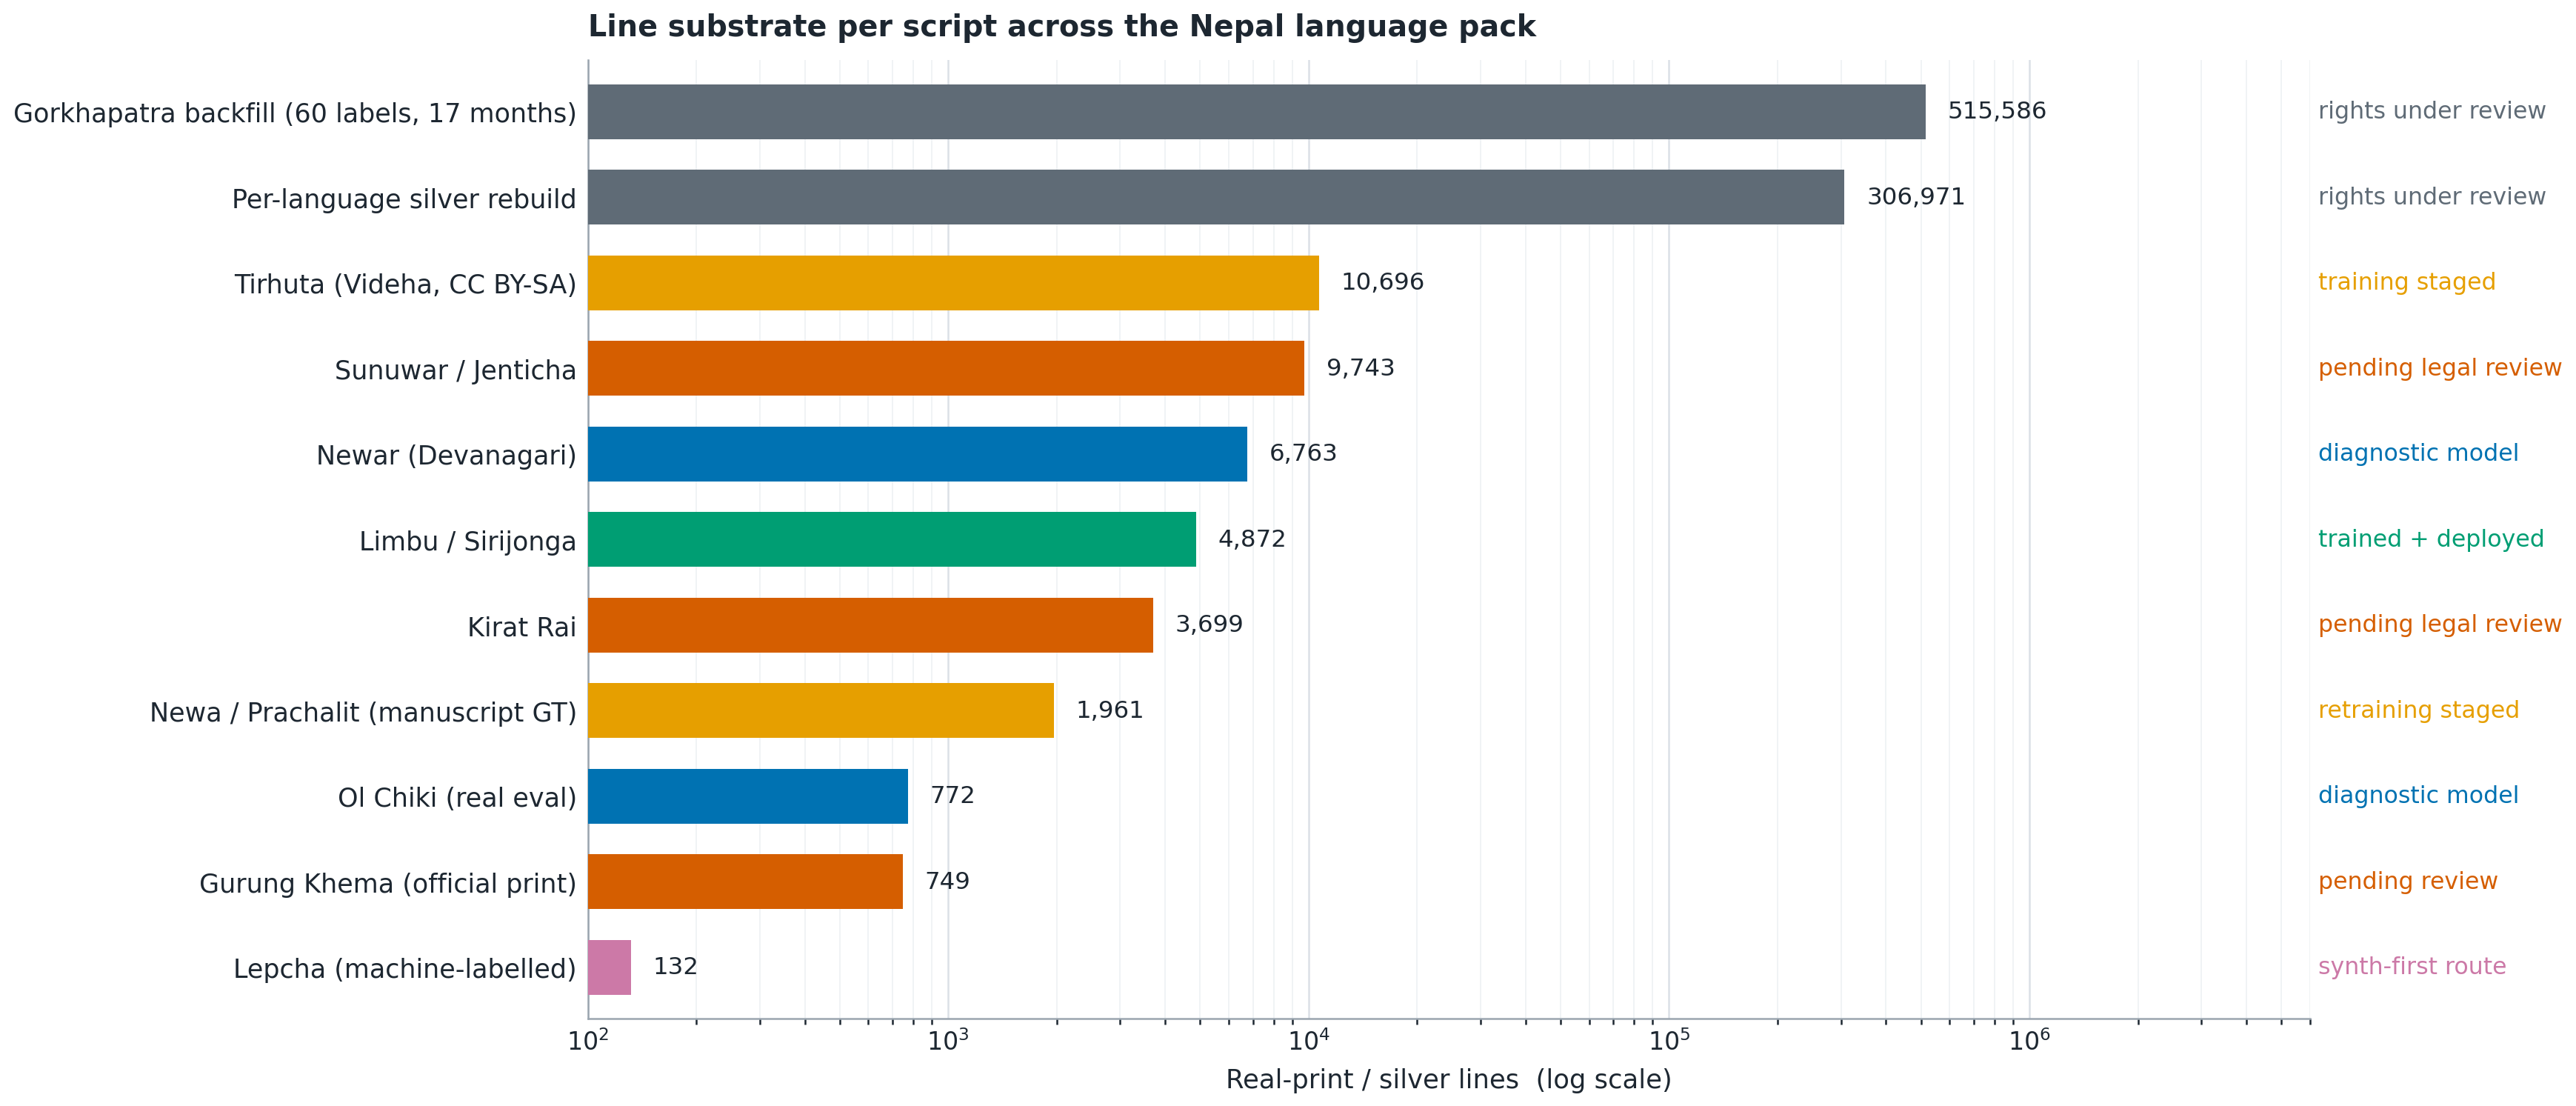
\includegraphics[width=1\linewidth,height=\textheight,keepaspectratio]{figures/language-pack-status.png}
\caption{Real-print and silver line substrate per script, with pipeline
status. Counts are read from the recorded pack artifacts at figure-build
time. All rows are mechanical silver or diagnostic substrate, not
human-reviewed ground truth.}
\end{figure}

\begin{multicols}{2}

\subsubsection{10.1 Substrate at scale}\label{substrate-at-scale}

Gorkhapatra's \emph{Naya Nepal} archive rotates pages for more than
fifty languages. We applied the Limbu same-page rule to that archive at
two depths. A monthly backfill from March 2024 through July 2025
retained \textbf{515,586} converted silver lines with line-level
provenance. A separate per-language rebuild of the current archive
retained \textbf{306,971} lines across the 50-language registry. The
collections overlap and have not been deduplicated against one another,
so adding the numbers would not give a corpus size.

These labels identify their pages, not necessarily the language of each
line. Nepali headings and other furniture appear on language pages, so
line-level language identification is required before training a
per-language recognizer. Gorkhapatra is Nepal's state-owned national
daily. An owner determination dated 2026-07-22 permits publication of
derived counts and metrics, but page and crop redistribution remains on
hold pending a formal license statement.

\subsubsection{10.2 Newar, the second
language}\label{newar-the-second-language}

We chose Newar (Nepal Bhasa) as the second focus language because its
Devanagari route could exercise the full Limbu workflow quickly. A
publication-date split produced 4,096 training, 1,528 development, and
1,139 test lines from Gorkhapatra pages. After a storage failure,
however, the recovered labels lacked the row-level provenance needed to
reconstruct that isolation.

On the frozen test, generic \texttt{deva-v2}, which was not trained on
Newar, records 6.223\% codepoint CER. The warm-started
\texttt{newar-ft-v1} records \textbf{4.655\%} codepoint CER, 9.569\%
grapheme CER, and 24.50\% exact-line accuracy. The same non-oracle page
path used for Limbu gives 19.92\% page codepoint CER, 91.16\% detection
F1, and 9.05\% matched-line codepoint CER on 19 pages. The gap between
matched-line and page results points toward recognition and crop-domain
error more than reading order, but the evidence is too compromised for a
firm attribution.

The later audit found whitespace artifacts in converted labels, 18 exact
cross-split matches, 575 rows sharing a 16-codepoint substring across
the train/evaluation boundary, missing provenance fields, and an open
rights review. It marks the pack not admitted for claims. The useful
result here is procedural: the shared path produced a working Newar
diagnostic within days, and the audit then stopped it from becoming an
accuracy claim. Section 10.5 covers the more difficult native-script
routes.

\subsubsection{10.3 Scripts with staged training, pending
review}\label{scripts-with-staged-training-pending-review}

Four other scripts have real-print material and staged training sets,
but no training run. Their archives are pinned by hash, development data
are split by issue or page, and filenames, line identities, and
normalized labels have zero train/development intersection.

\textbf{Tirhuta.} The Maithili e-zine \emph{Videha} publishes a parallel
Tirhuta edition. Its archived issues carry uploader-applied CC BY-SA 4.0
statements, recorded per issue with attribution, but the PDFs use legacy
glyph-substitution fonts. Recovering that mapping, including a 149-entry
conjunct extension, yielded \textbf{10,696} clean real lines. To our
knowledge, this is the first real-print Tirhuta OCR substrate at this
scale. The staged fine-tune split contains 9,765 training and 844
development rows, with a complete issue held out. A separate
48,960-image synthetic pack uses an openly licensed Tirhuta font and
audited degradation profiles. The pretrain-then-fine-tune chain is
ready, but no model has been trained and no GPU run is yet approved.

\textbf{Ol Chiki.} A magazine evaluation pack retains \textbf{772} clean
lines from 895 candidates; a dark-pixel guard removed 123 blank or
nearly blank renders. The synthetic-trained v2 recognizer scores
\textbf{8.26\%} codepoint CER and 20.34\% exact-line accuracy on it. We
withdrew that model from claim use after an asset audit found that its
training fonts came from the evaluation edition. A new
public-source-only v3 training set has 5,307 images: 242 real training
lines from a public-domain-marked issue, 5,000 synthetic replays, and 65
real development lines. It awaits native review. Santali OCR already
exists elsewhere, so this work is language-pack coverage rather than a
first-ever claim.

\textbf{Sunuwar and Kirat Rai.} Government-hosted Sikkim Herald editions
yielded \textbf{9,743} clean Sunuwar/Jenticha lines and \textbf{3,699}
Kirat Rai lines. Their legacy-font converters are grounded in the
relevant encoding proposals and leave no unresolved units. The Sunuwar
split has 8,422 training and 514 development lines; Kirat Rai has 2,865
and 193. Both training sets remain unused while legal review determines
whether the State Portal permission covers model training.

\subsubsection{10.4 Negative results that redirected
routes}\label{negative-results-that-redirected-routes}

Two failures forced us to change route. The Lepcha converter returned no
lines from 18 Sikkim Herald editions. Inspection showed why: the article
bodies are raster images, not live PDF text, so no font converter can
recover them. The Lepcha path now starts with synthesis and a
\textbf{132}-crop machine-labelled diagnostic that is explicitly
ineligible for claims. The harvester also records raster article bodies
as a distinct source type.

The manuscript-Newa recognizer failed even on its training data for a
different reason. Its mobile backbone always pools the sequence to 40
CTC timesteps, whereas 95.7\% of the manuscript lines contain more than
40 characters. CTC cannot emit more labels than timesteps; additional
examples could not solve the mismatch. We also found label defects, but
they were secondary. A T=200 configuration now passes shape and loss
checks, and a leakage-filtered 1,961-row training set has a sealed
635-line holdout; retraining awaits an approved run. These failures
matter because each one identifies a mechanism and changes the next
experiment.

\subsubsection{10.5 Source-first discipline for the hardest
scripts}\label{source-first-discipline-for-the-hardest-scripts}

For Gurung Khema and native-script Newar, the work stops at the source
audit. Official Sikkim Herald Gurung Editions contain running Gurung
Khema print, overturning our earlier belief that only synthetic material
was available; independent verification of the source is still in
progress. A converter grounded in the Unicode proposal can mechanically
convert \textbf{749} of 759 candidate lines, but none is used yet:
provenance checks, native pixel-label review, and split and leakage
checks remain unfinished.

Newar is represented by four writing-system profiles: Prachalit (encoded
Newa), Bhujimol, Ranjana, and Devanagari. Bhujimol has no distinct
Unicode encoding, and Ranjana remains unencoded, so neither can simply
reuse the Prachalit route without a transcription policy. We catalogued
and acquired Bhujimol and Ranjana manuscript groups only from
institutional archives with explicit reuse statements, hashed each
image, and prepared blank worksheets for qualified verification. There
are still no reviewed labels, models, or metrics. In this registry,
``supported'' can mean that input and output semantics are defined; it
does not imply that a recognizer exists.

\subsubsection{10.6 What the pipeline does not
claim}\label{what-the-pipeline-does-not-claim}

No result in this section is claim-grade. The intended near-term system
has one Sirijonga recognizer, one shared Devanagari recognizer, and
script-specific experts added only after rights-cleared, natively
reviewed evaluation becomes available. What exists today is the
auditable substrate: sources, converters, staged training sets,
diagnostics, and explicit refusals to run unreviewed models. Each
remaining model still has to earn its place per language, script, and
domain slice.

\subsection{11. Research Agenda}\label{research-agenda}

The next experiments should close a specific gap in the system, reuse
frozen evidence where appropriate, and keep every correction tied to its
source. We order that work below by dependency rather than novelty.

\subsubsection{11.1 Stage A: human-grounded Sirijonga
evaluation}\label{stage-a-human-grounded-sirijonga-evaluation}

The first priority is a Sirijonga benchmark reviewed by fluent readers.
Review should begin with the three date-separated line and page sets,
preserving both the original silver labels and the corrected text.
Disagreements and their resolution need to be recorded. The benchmark
can then grow to at least 30 independent pages from newspapers and
books, split by source rather than random crops.

The release should include reviewer agreement or an adjudication record,
rare-character and punctuation coverage, and a near-duplicate audit.
Scoring the same predictions against both silver and corrected
references will show how much PDF text-layer noise currently helps or
hurts the result.

Rights work runs in parallel. If page images and crops cannot be
redistributed, any release of derived metrics or reproduction recipes
must use an explicitly reviewed basis and state that boundary. The
rights decision determines the release design.

\subsubsection{11.2 Stage B: genuine Devanagari-written
Limbu}\label{stage-b-genuine-devanagari-written-limbu}

Work on the second writing system starts with source inspection.
Candidate pages must visibly use Devanagari, contain Limbu language, and
have line references aligned to those pixels. The manifest must say
whether the task is same-script OCR or Sirijonga-to-Devanagari
transcription.

Once that pack is frozen, generic \texttt{deva-v2} becomes the baseline.
Training or adaptation then uses source-group-separated data. Automatic
routing should be tested only after both scripts have relevant page
evidence, ideally on books or pages that genuinely mix them. Emitting
Devanagari characters is not enough; the model must read
Devanagari-written Limbu.

\subsubsection{11.3 Stage C: real-book and phone-capture
robustness}\label{stage-c-real-book-and-phone-capture-robustness}

Newspaper lines understate the difficulty of books and phone
photographs. The next set needs skew, perspective, page curvature,
uneven light, damaged print, bleed-through, varied fonts, marginalia,
headings, page numbers, illustrations, and changing layouts. Capture
preparation and OCR should be scored together so that a rectification
error is not attributed to recognition.

Detection recall and missed-line recovery deserve particular attention.
Layout rules must be chosen without reference text and tested across
page families. Multi-page runs should resume deterministically and
handle duplicate or out-of-order captures. At least one trial should
cover a complete work rather than a set of unrelated pages.

\subsubsection{11.4 Stage D: human-centered evaluation and iterative
learning}\label{stage-d-human-centered-evaluation-and-iterative-learning}

The review interface is itself part of the experiment. A study should
measure:

\begin{itemize}
\tightlist
\item
  raw and post-review CER/WER;
\item
  line precision, recall, F1, and reading-order accuracy;
\item
  missed, extra, empty, and falsely confident lines;
\item
  percentage of lines and pages routed to review;
\item
  correction time per page and per thousand characters;
\item
  recapture and resegmentation frequency; and
\item
  reviewer agreement and fatigue.
\end{itemize}

Queue policies can then be compared at a fixed final-quality target.
Sending fewer rows to review is not an improvement if more text
disappears. Accepted corrections enter versioned training packs only
after audit, keeping the deployment loop a controlled source of new
data.

\subsubsection{11.5 Stage E: document structure and selective
fallback}\label{stage-e-document-structure-and-selective-fallback}

The current pages are mostly dense newspaper text. Books add tables,
figures, captions, lesson layouts, and other page furniture.
Structure-aware references should test reconstruction in Markdown and
JSON. A larger document model may handle selected hard regions, but we
need to report how often it runs, why it was triggered, its latency, and
the measured gain. If it processes every page, it should be evaluated as
a different system.

\subsubsection{11.6 Stage F: gated transfer across the language
pack}\label{stage-f-gated-transfer-across-the-language-pack}

Section 10 shows that the reusable components already produce sources,
converters, staged training sets, and diagnostics for several scripts.
The remaining steps have a fixed order. First, resolve the Sikkim Herald
legal question; the Gorkhapatra determination is already in the ledger.
Next, obtain native review for each staged evaluation set. Only then run
the approved training chains---Tirhuta pretraining and fine-tuning, Ol
Chiki v3, and Newa T=200---against frozen, edition-disjoint tests.

Admission happens one language, script, and domain slice at a time.
Sharing a codepoint range or using a generic Devanagari model does not
establish language or visual coverage. This paper makes no claim-grade
accuracy statement for any language, including Limbu.

\subsection{12. Limitations, Rights, and Community
Governance}\label{limitations-rights-and-community-governance}

\subsubsection{12.1 Silver references and source
concentration}\label{silver-references-and-source-concentration}

The largest numerical limitation is reference quality. Same-PDF
alignment is better than pairing a page with unrelated website text, but
converted text layers still contain encoding, ordering, grouping, and
normalization errors. A model trained on one publisher may learn that
publisher's typography and PDF artifacts. Three held-out pages cannot
represent other books, publishers, fonts, historical periods, or camera
conditions.

The previous deployment is an operational comparator, not a broad
baseline suite. Comparisons with other OCR systems should wait for a
frozen, rights-cleared, human-reviewed image set and use exactly the
same pixels.

\subsubsection{12.2 Incomplete two-writing-system
evidence}\label{incomplete-two-writing-system-evidence}

Both routes exist in the interface, but only Sirijonga has a surviving
Limbu-specific result. The presence of a Devanagari model is not
evidence about Devanagari-written Limbu. The curriculum mistake is a
concrete example of why we now inspect pixels and separate manifest
fields before assigning a sample to that branch.

\subsubsection{12.3 Rights and release
boundaries}\label{rights-and-release-boundaries}

The licensing ledger records an owner determination dated 2026-07-22 for
Gorkhapatra, Nepal's state-owned national daily. It permits the derived
counts and metrics reported here, not redistribution of pages or crops.
The paper uses artifact-derived diagrams while a formal
pixel-redistribution license remains open. That determination does not
cover the rest of the pack. Sikkim Herald training sets remain unused
while the State Portal permission is reviewed for training use. Only the
Videha Tirhuta source has recorded per-issue CC BY-SA 4.0 statements
with attribution. Any later data or model release must retain source
provenance and state precisely which material its rights basis covers.

\subsubsection{12.4 Language-pack
boundaries}\label{language-pack-boundaries}

The language-pack numbers add script-specific problems to those
limitations. Many silver lines are attributed to a page but not verified
for language. The Newar pack has cross-split leakage and missing row
provenance. The Ol Chiki diagnostic used fonts derived from its
evaluation edition and was withdrawn from claim use. A per-language
Devanagari scorecard lost its backing artifacts in the storage failure
and is omitted. No language in the pack has a native-reviewed evaluation
set; the per-script review records in Section 10 govern what can
currently be said.

\subsubsection{12.5 Community validation}\label{community-validation}

Metrics cannot settle linguistic correctness, preferred script names, or
community acceptance. Fluent Limbu readers need a role in benchmark
review, error taxonomy, interface testing, and release decisions. Their
corrections and disagreements should remain visible instead of
disappearing into one final string. The practical question is whether
the output helps people search, edit, teach from, and preserve Limbu
documents---not whether it merely contains Unicode.

\subsubsection{12.6 Reproducibility
boundary}\label{reproducibility-boundary}

The build regenerates the figures and checks source counts, splits,
metrics, model hashes, runtime paths, and source-representation findings
against local artifacts. It does not repeat the L4 training run. The
training bundle, configuration, checkpoint, inference export,
predictions, page records, and scores remain available for inspection.

\subsection{13. Conclusion}\label{conclusion}

LimbuOCR is now an operational research platform that turns page images
and PDFs into editable, structured, reviewable Limbu text. The measured
Sirijonga route records 0.474\% codepoint CER, 0.979\% grapheme CER, and
85.92\% exact-line accuracy on a three-date silver test. Starting from
the complete pages, it records 2.575\% codepoint CER with 96.85\%
detection F1. The same source and release workflow has also produced
large silver collections, converters, staged training sets, a Newar
diagnostic, and two useful negative results across the Nepal language
pack.

Those artifacts mark the starting point, not the finish. The Sirijonga
labels need native validation and broader book and camera coverage.
Devanagari-written Limbu needs verified pages of its own. Every other
language remains behind its rights and native-review gates. The
reading-order correction and the withdrawn curriculum result show why
these boundaries belong in the method, not in a footnote. The next
meaningful measure is review burden on a complete book: how much time
the system saves while keeping missed text and uncertain lines visible.

\phantomsection\label{refs}
\begin{CSLReferences}{1}{0}
\bibitem[\citeproctext]{ref-agarwal2024survey}
Agarwal, Milind, and Antonios Anastasopoulos. 2024. {``A Concise Survey
of {OCR} for Low-Resource Languages.''} In \emph{Proceedings of the 4th
Workshop on Natural Language Processing for Indigenous Languages of the
Americas}, 88--102. Association for Computational Linguistics.
\url{https://doi.org/10.18653/v1/2024.americasnlp-1.10}.

\bibitem[\citeproctext]{ref-cui2025paddleocr3}
Cui, Cheng, Ting Sun, Manhui Lin, Tingquan Gao, Yubo Zhang, Jiaxuan Liu,
Xueqing Wang, et al. 2025. {``{PaddleOCR 3.0} Technical Report.''}
\emph{arXiv Preprint arXiv:2507.05595}.
\url{https://arxiv.org/abs/2507.05595}.

\bibitem[\citeproctext]{ref-gebru2021datasheets}
Gebru, Timnit, Jamie Morgenstern, Briana Vecchione, Jennifer Wortman
Vaughan, Hanna Wallach, Hal Daumé III, and Kate Crawford. 2021.
{``Datasheets for Datasets.''} \emph{Communications of the ACM} 64 (12):
86--92. \url{https://doi.org/10.1145/3458723}.

\bibitem[\citeproctext]{ref-graves2006ctc}
Graves, Alex, Santiago Fernández, Faustino Gomez, and Jürgen
Schmidhuber. 2006. {``Connectionist Temporal Classification: Labelling
Unsegmented Sequence Data with Recurrent Neural Networks.''} In
\emph{Proceedings of the 23rd International Conference on Machine
Learning}, 369--76. Association for Computing Machinery.
\url{https://doi.org/10.1145/1143844.1143891}.

\bibitem[\citeproctext]{ref-li2022ppocrv3}
Li, Chenxia, Weiwei Liu, Ruoyu Guo, Xiaoting Yin, Kaitao Jiang, Yongkun
Du, Yuning Du, et al. 2022. {``{PP-OCRv3}: More Attempts for the
Improvement of Ultra Lightweight OCR System.''} \emph{arXiv Preprint
arXiv:2206.03001}. \url{https://arxiv.org/abs/2206.03001}.

\bibitem[\citeproctext]{ref-limbu2024heritage}
Limbu, Sumi. 2024. {``Linguistic Heritage in Digital Landscape: A
Collective Memory of Indigenous Script.''} Master of Design thesis,
University of Arkansas. \url{https://scholarworks.uark.edu/etd/5325/}.

\bibitem[\citeproctext]{ref-mitchell2019modelcards}
Mitchell, Margaret, Simone Wu, Andrew Zaldivar, Parker Barnes, Lucy
Vasserman, Ben Hutchinson, Elena Spitzer, Inioluwa Deborah Raji, and
Timnit Gebru. 2019. {``Model Cards for Model Reporting.''} In
\emph{Proceedings of the Conference on Fairness, Accountability, and
Transparency}, 220--29. Association for Computing Machinery.
\url{https://doi.org/10.1145/3287560.3287596}.

\bibitem[\citeproctext]{ref-muehlberger2019transkribus}
Mühlberger, Günter, Louise Seaward, Melissa Terras, Sofia Ares Oliveira,
Vicente Bosch, Maximilian Bryan, Sebastian Colutto, et al. 2019.
{``Transforming Scholarship in the Archives Through Handwritten Text
Recognition: Transkribus as a Case Study.''} \emph{Journal of
Documentation} 75 (5): 954--76.
\url{https://doi.org/10.1108/JD-07-2018-0114}.

\bibitem[\citeproctext]{ref-poncelas2020postediting}
Poncelas, Alberto, Mohammad Aboomar, Jan Buts, James Hadley, and Andy
Way. 2020. {``A Tool for Facilitating {OCR} Postediting in Historical
Documents.''} In \emph{Proceedings of LT4HALA 2020 -- 1st Workshop on
Language Technologies for Historical and Ancient Languages}, 47--51.
European Language Resources Association (ELRA).
\url{https://aclanthology.org/2020.lt4hala-1.7/}.

\bibitem[\citeproctext]{ref-sharma2024voltage}
Sharma, Prawaal, Poonam Goyal, Vidisha Sharma, and Navneet Goyal. 2024.
{``{VOLTAGE}: A Versatile Contrastive Learning Based {OCR} Methodology
for Ultra Low-Resource Scripts Through Auto Glyph Feature Extraction.''}
In \emph{Proceedings of the 18th Conference of the European Chapter of
the Association for Computational Linguistics}, 881--99. Association for
Computational Linguistics.
\url{https://doi.org/10.18653/v1/2024.eacl-long.53}.

\bibitem[\citeproctext]{ref-smith2007tesseract}
Smith, Ray. 2007. {``An Overview of the Tesseract OCR Engine.''} In
\emph{Proceedings of the Ninth International Conference on Document
Analysis and Recognition}, 629--33. IEEE Computer Society.
\url{https://research.google/pubs/an-overview-of-the-tesseract-ocr-engine/}.

\bibitem[\citeproctext]{ref-unicode17limbu}
Unicode Consortium. 2025a. {``The Unicode Standard, Version 17.0:
Chapter 13, Limbu.''} Unicode Standard.
\url{https://www.unicode.org/versions/Unicode17.0.0/core-spec/chapter-13/}.

\bibitem[\citeproctext]{ref-uax29}
---------. 2025b. {``Unicode Text Segmentation.''} Unicode Standard
Annex \#29. \url{https://www.unicode.org/reports/tr29/}.

\end{CSLReferences}

\end{multicols}

\end{document}
